% to-do
% Add more to introduction, explain more about general binaries the process of how it works
% 
% add more regarding common binaries

% Captions on all graphics

% xray accretion section

% vela x-1 properties

% good excerpt on CEE evolution over time
%As mentioned before, the common envelope evolution (CEE) has been first proposed in 1976 to account for the origin of cataclysmic variables (CVs). CVs are binaries consisting of a WD with a typical mass of around and an MS companion star with a typical mass of , in which the MS star fills its Roche lobe and undergoes the mass transfer. They typically have an orbital period of 1 to 10 h. Regarding the origin of CV systems, the question is how to form such massive WDs in such a close binary system with an orbital period of a few hours. According to the stellar evolution theory, massive WDs could be formed from cores of red giants (or supergiants) before their envelopes are removed. In this case, the orbital period of a binary system needs to be long enough to keep the red giant (or supergiant) within its Roche lobes until a massive core is formed. Then, a mechanism is needed to drastically reduce the orbital period to a few hours consequently to match the observed periods of CVs. This therefore leads to the proposal of CEE (e.g. [198], [223], [224]). By adopting the CE scenario, the origin of V 471 Tau was successfully explained [198], i.e., a detached binary in the Hyades cluster which has a WD and a K-type dwarf, with an orbital period of . This binary system is expected to evolve into a CV system within a few yr.

% Add section explaining what causes binaries to draw closer to eachother, why its needed, etc etc, 

% GwR, Mass Loss, and Magnetic braking

% things to figure out

% cause of the line in contact binaries

% distribution of masses for contact binaries (cant due to small quantity and the nature of trying to observe contact binares)

% more history lesson stuff?

% The near-circular orbit of Vela X-1 prompts the questions whether the first mass transfer in the system might have lead to a Common Envelope (CE) phase (Paczynski 1976). Even though many uncertainties remain on the detailed physical processes involved in CE evolution, their occurrence is typically inferred from an evolutionary necessity (e.g., Ivanova et al. 2013). CE stages are thought to occur for unstable RLOF and help to shrink and circularize the orbit, at least if the system can eventually eject the envelope and avoid merging. However, CE stages are unlikely to occur for the first mass transfer stage in an HMXB




% suggestions 
% less acrynoms 
    % MT

    % the following sections will describe rlo ....

    % simplier graphic for the binary evolution
    % LaGrangian point explination and section
    % wind accretion and atmospheric RLO~\ref{atmosperhicrlo}
    % system fully filling up gravitional potetional and then lossing that mass itself. 
    % common envolope and stable evolution more

% discussion
    % Further research
    % where do we go?
    % more captions 
    % binary evolution
        % this ilustrates the complexity of binary evolution
    % Explain POSYDON more 
    % make graphs bigger and such

    

% Standerize the section orders RLO, detached, contact.

\documentclass[12pt, a4paper]{article}
\usepackage{titlesec}
\usepackage{graphicx}
\usepackage{geometry}
\usepackage{abstract}
\usepackage[T1]{fontenc}
\usepackage{lipsum}
\usepackage{tabularx}
\usepackage{float}
\usepackage{amssymb}
\usepackage{hyperref}
\usepackage[
  backend=biber,
  sorting=none,
%   style=mla
]{biblatex}
\addbibresource{sources.bib} 
\usepackage[labelfont=bf, labelsep=colon, textfont=it]{caption}


\renewcommand{\abstractnamefont}{\normalfont\Large\bfseries} 
\renewcommand{\arraystretch}{1.2}

\titleformat{\section}
  {\normalfont\Large\bfseries\centering} % Formatting for the section title
  {} % Empty label (hides the number)
  {0pt} % No spacing before title
  {} % No additional formatting

\titleformat{\subsection}
    {\normalfont\Large\bfseries\centering}
    {\thesubsection}
    {.5em}
    {}
\titleformat{\subsubsection}
    {\normalfont\small\bfseries\centering}
    {\thesubsubsection}
    {.5em}
    {}



\title{Mass Transfer in Binary Stars}
\author{Pierson Lipschultz\thanks{Advisor: Joseph DalSanto}}

\date{\today}
\begin{document}
\maketitle
\begin{abstract}
    \normalsize
    In this paper, I investigate the properties of mass transfer in binary stars. I utilize the Roche Lobe model to categorize the systems in detached, semi-detached, and contact. I then investigate the process of mass transfer within those types of systems. I use the systems Vela X-1, V404 Cygni, and W Ursae Majoris as examples of each type of system, using data from each. I further corraborate this data from a dataset generated from POSYDON of a million binary stars. I found the local populations on an HR diagram of each system and found the main causes of mass transfer in detached systems to be wind accretion, semi-detached to be Roche Lobe overflow, and contacts to be direct mass sharing. Additionally, I found properties in both W UMa and V404 Cygni which warrant further investigation.

\end{abstract}

\section{Introduction} % amaybe include a section on x-ray emission???

    Most of the stars we see in the night sky are not actually single stars, instead consisting of multiple stars orbiting a common center of mass. A pair of such stars is called a binary. These binaries are formed in the same nature of single stars, that being from a molecular cloud. However, due to instability in the formation process, two or more stars are formed instead of one \parencite{Offner_2016}. The stars in these binary pairs will a have a different evolutionary track on an HR diagram than a single star, as it is highly likely for the two stars to interact at some point during their life due to their proximity in formation~\parencite{TaurisvandenHeuvel+2023}. As these stars evolve and interact with each other, it drastically affects their evolution (see fig.~\ref{fig:binary_evolution_flowchart}).


    \subsection{Mass Transfer in Common Binaries}~\label{MassTransferinCommon}
    In systems with small orbital separations, a process called mass transfer can occur~\parencite{TaurisvandenHeuvel+2023}. This is where one star called a donor will ``donate'' mass to the other star, called the accretor as gravity draws material off of the donor. This is likely to occur at some point during the binaries' lifespan, leading to different evolutionary outcomes as compared to single star evolution~\parencite{TaurisvandenHeuvel+2023} (see fig.~\ref{fig:binary_evolution_flowchart}). However, depending on the duration of mass transfer and the star type, this process can be hard to detect observationally. Because of this, a large quantity of studies have been conducted on binaries with more extreme star types, such as neutron stars or black holes, where the process of mass transfer leads to much more pronounced effects. This is because as the mass is transferred to the black hole or neutron the process leads to a large spike in X-ray emissions (sect.~\ref{XrayAccretion}), which can more easily measured as compared to the mass transfer process between, for example, a red giant and a main sequence star, which have little to no x-ray emission.
    
    In figure~\ref{fig:binary_evolution_flowchart} we see a slice of a high level overview regarding the types of binary star evolution. In the evolution of binaries' stars there are many different stages which the system will evolve in and out off, with each of these stages having different outcomes based on the systems properties.

    \newgeometry{left=0.75in, right=0.75in, top=0.5in, bottom=0.5in}
    \vspace*{\fill}
    \begin{figure}[H]
        \centering
        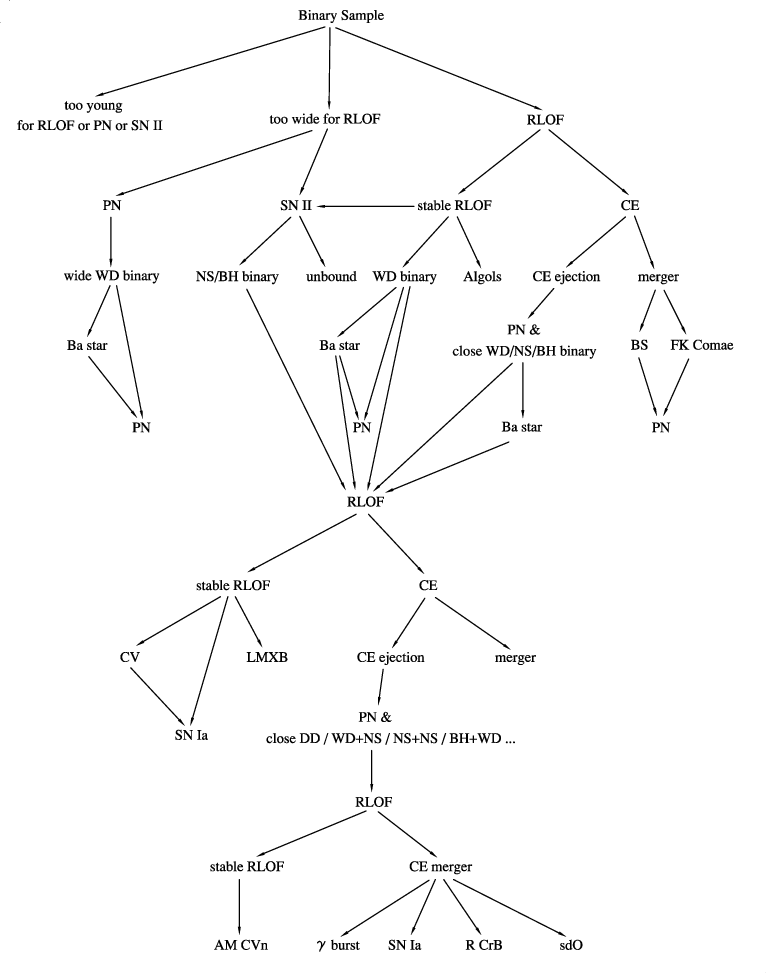
\includegraphics[width=\textwidth]{figs/reused-figs/Han_BinaryEvolFlowchart.png}
        \caption{A heavily simplified flowchart of binary evolution. Reprint from \parencite{Han_2008}. See much more in depth version in \parencite{Chen_2024}}.
        \label{fig:binary_evolution_flowchart}
    \end{figure}
    \vspace*{\fill}
    \restoregeometry

    \subsection{Roche Lobe Model} \label{RLModel} % maybe find the orignal rlm paper and use that to elaborate? it feels weird to not talk more here about this, however, it would be very easy to just spend forever talking about it. 
        The Roche Lobe (RL) model was proposed by Édouard Roche and defines the gravitational potential of a binary through a simple model by visualizing the region around a star where it can hold onto its mass (i.e. great enough gravitational potential). If one of the stars in the binaries' mass overflows said lobe, it will transfer mass to its binary pair. This model can be used to classify binary star populations into various populations, including detached binaries (where neither star has filled their potential), semi-detached systems (where one star has filled its potential, leading to mass transfer to an accretor) and contact binaries (where both stars have filled their potentials), 

    \vspace*{\fill}
    \begin{figure}[H]
        \centering
        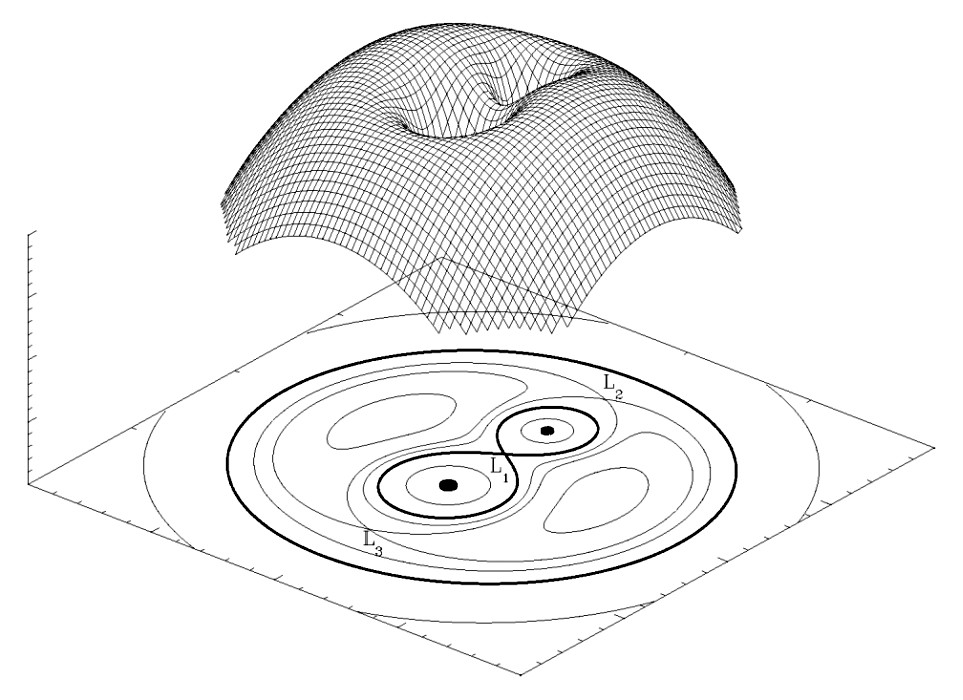
\includegraphics[width=\textwidth]{figs/reused-figs/Wiki-RochePotential.jpg}
        \caption{ A 3D representation of the gradient of the Roche lobe. In this figure the potential has been mapped to a height, creating a 3D model. Note the main sections of potential around the stars.}
        \label{fig:Roche_potential}
        \textit{\small Reprint from \parencite{vandersluys2005}}
    \end{figure}
    \vspace*{\fill}

        \subsection{Detached binaries}\label{DetachedBinary}

        \begin{figure}[H]
            \centering
            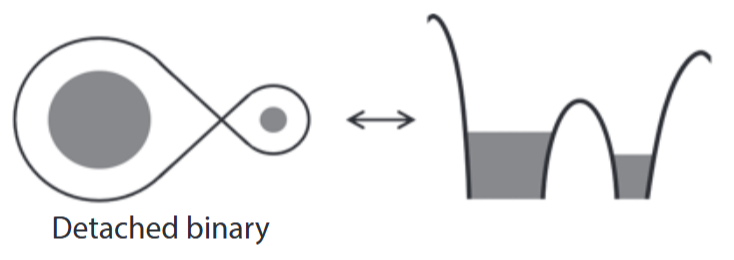
\includegraphics[scale = .4]{figs/reused-figs/Tauris_DetachedBinary.png}\\
            \textit{Reprint from~\parencite{TaurisvandenHeuvel+2023}}
            \caption{Graphic of the RL model with regard to how much potential is being filled in a detached binary. Note here that has both a `top-down' perspective and from the side.}
            \label{DetachedBinaryRL}
        \end{figure}

        Systems where neither star fills its potential fully (fig.~\ref{DetachedBinaryRL}) are called detached binaries. Despite the fact that these systems have not filled their Roche lobes, mass transfer is still possible through a processes called wind accretion (sect~\ref{WindAccretion}). We see this predominantly in systems called High Mass X-ray Binaries (HMXBs), where a supergiant star transfers mass to a compact object via wind accretion. This process leads to an increase in X-ray Emission (sect.~\ref{XrayAccretion}), which we can easily measure~\parencite{TaurisvandenHeuvel+2023}. It is important to note that despite the majority of HMXBs not experiencing full-blown RLO (sect\ref{RLO}) they tend to be very close to doing so~\parencite{TaurisvandenHeuvel+2023}. 

        I investigated the system Vela X-1~\parencite{Kretschmar_2021} (sect.~\ref{velax1introduction}) as an example of this as it is generally regarded as the ``archetypical wind accretor''~\parencite{Kretschmar_2021}. 

        \subsubsection{Wind Accretion Mass Transfer} \label{WindAccretion}
        Wind accretion is very different from normal mass transfer in a binary. All stars produce `wind,' i.e. mass which is pushed away from the star. Most stars cause a process called stellar wind, occurring when mass from the outer envelope is ejected at various speeds from the star. All stars experience varying strengths of stellar wind, with some winds having very high velocities, and others much lower.~\parencite{Lamers_1999} In binary stars this process allows mass that has escaped the donor to be transferred to the accreting star.

        \begin{figure}[H]
            \centering
            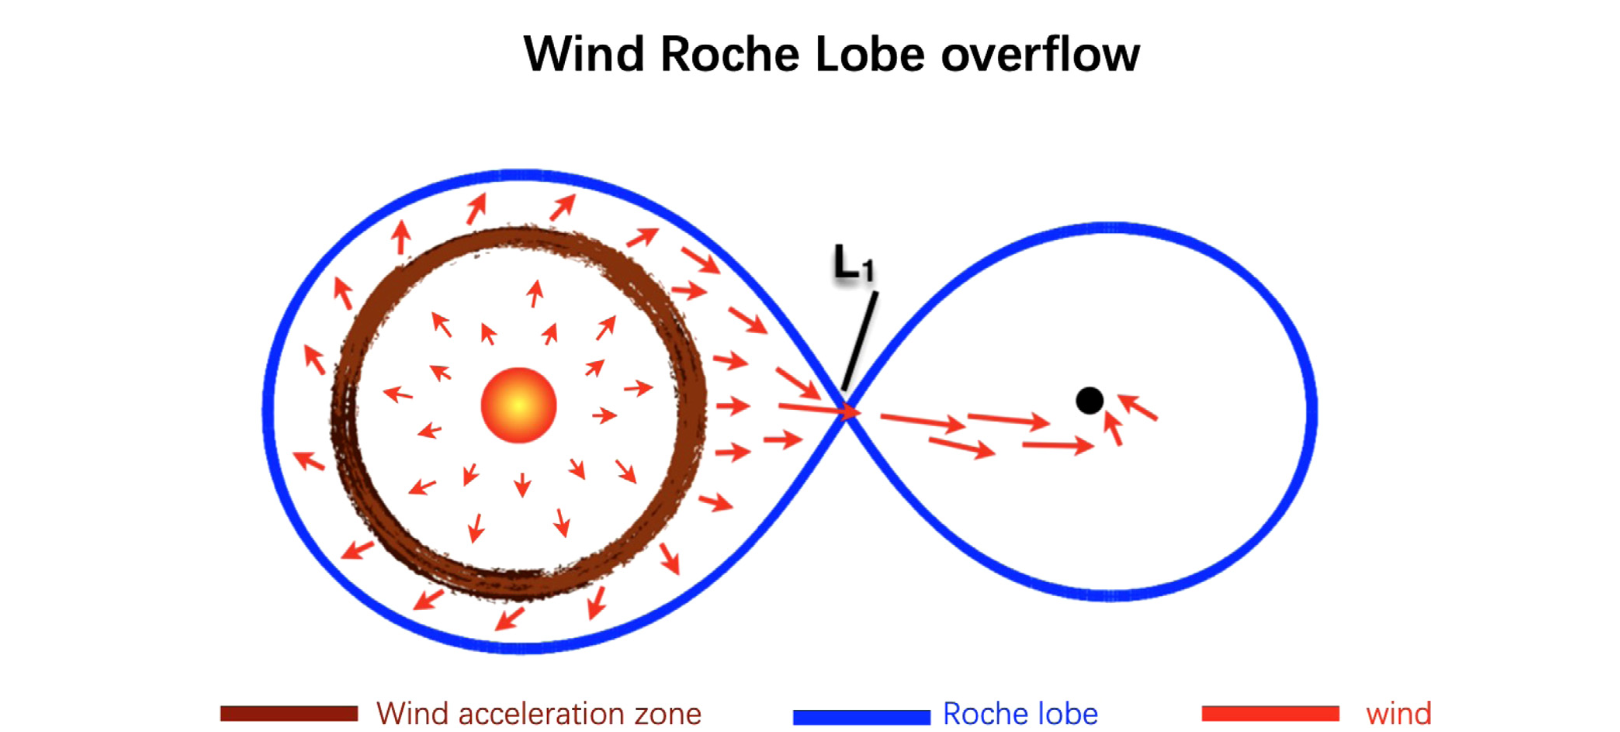
\includegraphics[width = .8\textwidth]{figs/reused-figs/Tauris_WindRocheLobeOverflow.png}\\
            \textit{Reprint from~\parencite{TaurisvandenHeuvel+2023}}
            \caption{Graphic of the RL model showing wind accretion. Note here that this shows a `top-down' perspective.}
            \label{fig:RLWindAccretion}
        \end{figure}
        
        \subsection{Semi-detached Binaries}\label{RLO} % maybe include equations??

        \begin{figure}[H] 
            \centering
            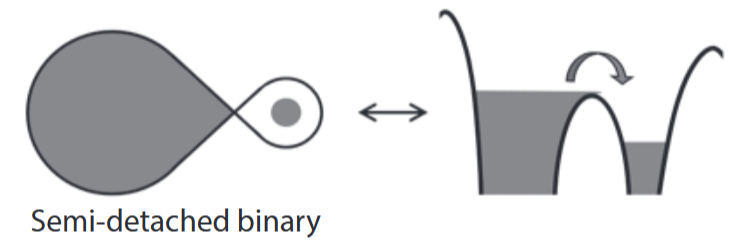
\includegraphics[scale = .4]{figs/reused-figs/Tauris_Semi-detachedBinary.png}
            \caption{\textit{Reprint from~\parencite{TaurisvandenHeuvel+2023}}}
            \label{SemidetachedRL}
        \end{figure}

        In systems where one star fully fills its RL (sect.~\ref{RLModel}, fig.~\ref{SemidetachedRL}) mass begins to be transferred to its binary partner. This is process is called Roche Lobe Overflow (RLO) and is defined by a donor and accretor star (sect.~\ref{MassTransferinCommon}). This is likely to happen at some point in a binaries' lifespan drastically affecting the course of evolution~\parencite{TaurisvandenHeuvel+2023}\parencite{Chen_2024}. Depending on the systems star types, masses, and orbital eccentricity, this process of mass transfer will either be stable or unstable. When this process if unstable, it leads to either another stage called common envelope (sect.~\ref{CommonEnvelope}) or a rapid merger \parencite{TaurisvandenHeuvel+2023}. However, if the process of mass transfer is stable, the two stars will remain detached, slowly exchanging mass~\parencite{Chen_2024}~\parencite{TaurisvandenHeuvel+2023}.

        We are able to observe this very commonly in Low Mass X-ray Binaries, where a donor star transferred mass to an accretor which is a compact object (a black hole or neutron star). This process produces X-rays (sect.~\ref{XrayAccretion}) which we can measure to understand the processes within the binary in greater detail.

        This process, similar to section~\ref{CommonEnvelope}, can be either stable or unstable. A large factor which determines this stability is the evolutionary stage of the donor star~\parencite{TaurisvandenHeuvel+2023}, as upon the onset RLO, some donors stars' radius will increase, leading to even more rapid RLO. This is primarily due to the nature of the stars' envelope, with radiative envelopes shrinking upon mass loss and convective envelope swelling \parencite{TaurisvandenHeuvel+2023}.
        
        In intermediate mass x-ray binaries, a system will survive this process of mass transfer if the unevolved or early stage donor star mass is between $2 < M_2/M_\odot < 5$ \parencite{TaurisvandenHeuvel+2023}. In low mass x-ray binaries (LMXBs) it is $M_2 \gtrsim 1.8 M_\odot$. Systems with $M_2 > 2$ Will be unstable for giant donors in later stage RLO~\parencite{TaurisvandenHeuvel+2023}.
        
        I used the system V404 Cygni (sect. \ref{V404Context}) with data from~\parencite{Bernardini_2016} and \parencite{Shahbaz_1994} as an example of this behavior, as its magnitude, proximity to Earth, and quantity of studies make it an ideal choice to understand how systems like it behave. 

        \subsubsection{Mass transfer through $L_1$} \label{L1MassTransfer}

        In this process of mass transfer, the mass will be transferred through the Lagrangian point $L_1$, as it is the point of lowest potential between them, as seen in figure~\ref{fig:Roche_potential}~\parencite{TaurisvandenHeuvel+2023}. The mass at $L_1$ feels an equal gravitational pull from both stars and thus requires no external force for the mass to be transferred. This rate of mass transfer is dependent on a pressure differential between the two stars \parencite{TaurisvandenHeuvel+2023}.

        \subsubsection{Atmospheric RLO} \label{atmosphericRLO}
        The Roche-lobe model assumes that ones the radius of the star crosses the Roche-lobe radius then mass transfer will start. However, this relies on the assumption that the edge of the star is completely sharp, which they are not. Instead, the star will have an atmosphere surrounding it. Once the radius of the atmosphere crosses the Roche-lobe radius, the atmosphere can begin to be transferred \parencite{TaurisvandenHeuvel+2023}. This is most relevant in HMXBs, where atmospheric accretion alone can make them strong x-ray sources. Once the photosphere of the star crosses the Roche-lobe radius `full-blown' RLO sets in.

        \subsection{Contact Binary}

        \begin{figure}[H]
            \centering
            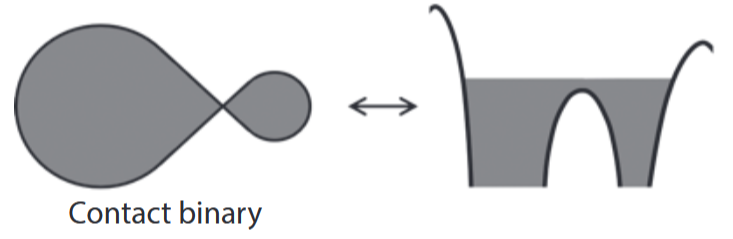
\includegraphics[scale = .4]{Figs/reused-figs/Tauris_ContactBinary.png}

            \caption{\textit{Reprint from~\parencite{TaurisvandenHeuvel+2023}}}
            \label{ContactBinaryRL}
        \end{figure}

        In binaries with prominent RLO it is possible for the donor star to fill up not just its own Roche Lobe, but the accretors' as well. This means that both the donors  potential and the gravitational accretors potential are filled. \parencite{TaurisvandenHeuvel+2023} As these stars have both fully filled their RL's, they transfer mass by physically being connected. This process of mass transfer can theoretically lead to mass transfer oscillating between which of the two stars is the donor (sect.~\ref{MassTransferOscillation}). 
        
        If both of the binaries' potentials are full, then donor star will then begin to fill up the systems total gravitational potential (i.e. the area between the two ridges in fig.~\ref{ContactBinaryRL}). This can lead to mass being loss from the system completely \parencite{TaurisvandenHeuvel+2023}, forming a formation similar to a planetary nebula.
        
        This process generally is not stable, as most stars this in stage generally are experiencing a brief stage of their evolution called common envelope (CE). (See section~\ref{CommonEnvelope}) However, in cases where it is stable, the stars will continue to evolve as one body (sect.~\ref{CommonEnvelopeStableEvoluton}).
        
        
        \subsubsection{Common Envelope (CE)}\label{CommonEnvelope}

            CE occurs in a binary system after runaway mass transfer which leads to the companion star being fully engulfed in the envelope of the donor \parencite{TaurisvandenHeuvel+2023}. This leads to forces which greatly reduce the orbital separation. This can either cause the two stars to merge within the environment or for the envelope to be ejected. The ejection of the envelope can allow for the two systems to remain detached, however, the stars are likely to merge in the process \parencite{TaurisvandenHeuvel+2023} (sect.~\ref{DetachedBinary}). This ejected mass can either orbit around the system, or be fully ejected from the system, which is a likely cause of planetary nebulae \parencite{TaurisvandenHeuvel+2023}. There are many questions about this process, as the short yet incredibly rapid evolution is incredibly difficult to model. \parencite{TaurisvandenHeuvel+2023}

        \subsubsection{Stable Evolution}\label{CommonEnvelopeStableEvoluton}
            In systems which are stable the stars will share mass and their shells will evolve in tandem, this process is called ``homogenous chemical evolution''. (See fig~\ref{fig:binary_evolution_flowchart} \parencite{Chen_2024}). As these stars transfer mass, their mass ratio ($q$) will oscillate around a value of $q=1$, eventually reaching $q_{min}$ at which point the stars will rapidly merge (see fig.~\ref{qEvolution}) \parencite{Pešta_2023}. These systems are rare as they require the two stars to have a similar mass \parencite{TaurisvandenHeuvel+2023}. 
            
        \begin{figure}[H]
            \centering
            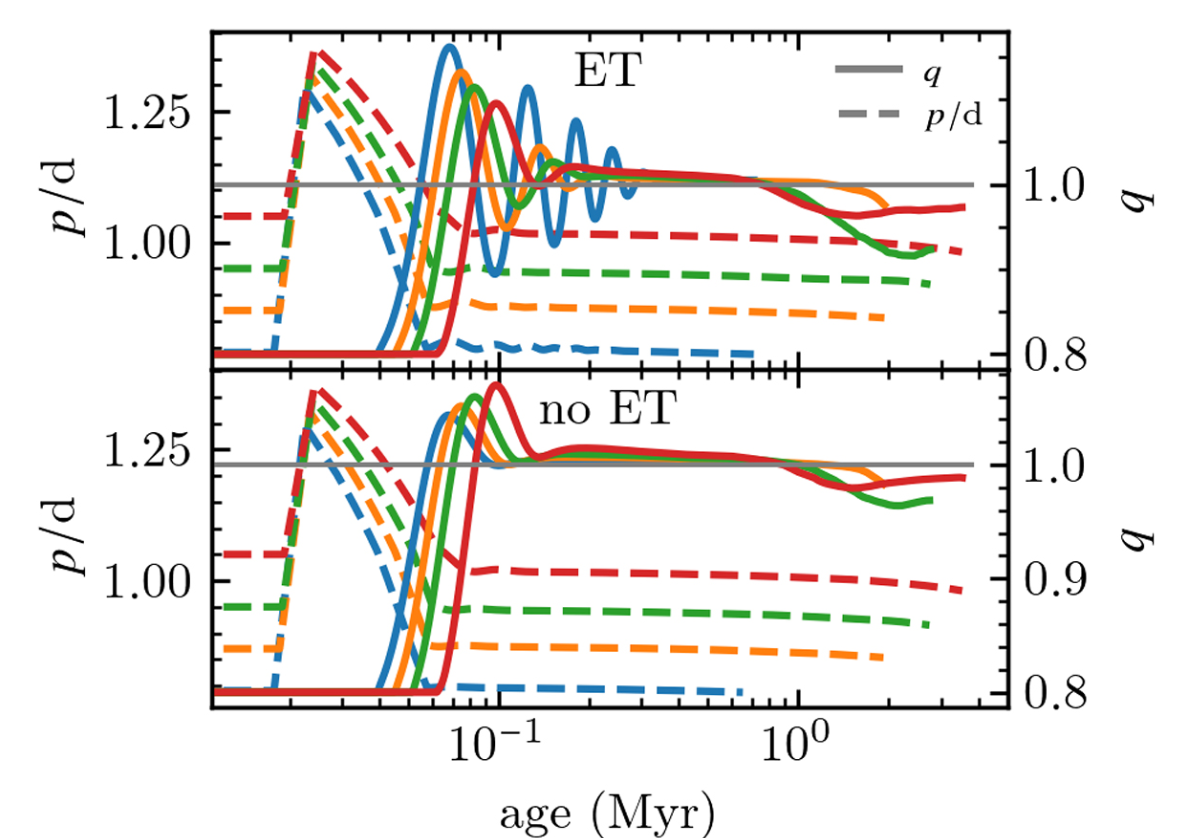
\includegraphics[scale = .3]{figs/reused-figs/q-ratio_evolution_farby.png}
            \caption{Reprinted from \parencite{Fabry_2025}. These graphs show the effects of modeling energy transfer(ET) on the systems' evolution.}
            \label{qEvolution}
        \end{figure}
        
        I used W Ursae Majoris (W UMa) (sect.~\ref{WUMaIntroduction}) as an example of CE systems, as it is used an example system in order to categorize these contact binaries as a whole.
    \subsection{X-ray Binaries} 
        \subsubsection{X-rays caused by accretion onto a compact object} \label{XrayAccretion}
            In 1962 the first X-ray binary was discovered by Riccardo Giacconi and colleagues. This system, Scorpius X-1, is so bright in x-ray that it actively raises ionization levels in Earths atmosphere when above the horizon. \parencite{TaurisvandenHeuvel+2023} \parencite{Giacconi_1962} In the years following, it was discovered that that Scorpius X-1 consisted of a normal star and neutron star. Since then, many thousands more have been discovered\parencite{Haardt_1993}.

            These x-rays are produced from the friction of in-spiralling matter, which causes it to become incredibly hot, with the inner disk reaching temperatures of $\geq$ 10 million K, causing it to emit a large amount of x-rays. In systems with a neutron star accretor, the surface of the neutron star itself will also emit a large amount of x-rays \parencite{TaurisvandenHeuvel+2023} (fig.~\ref{XrayAccretionMarkVis}). 

            \begin{figure} [H]
                \centering
                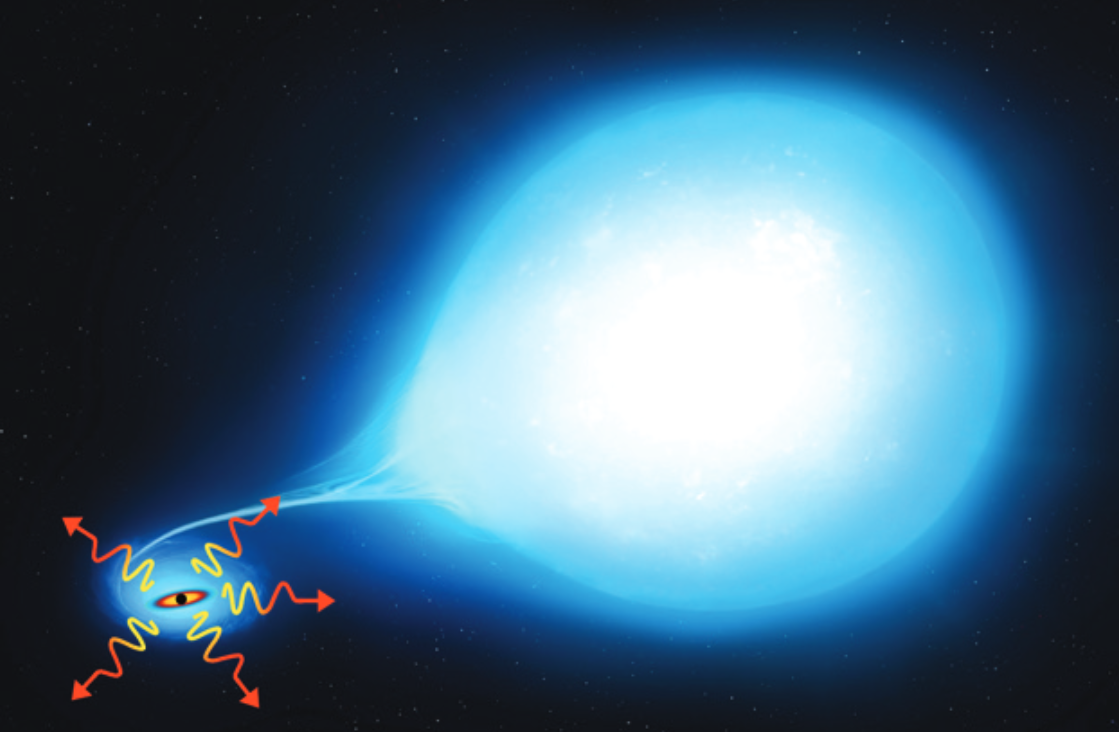
\includegraphics[width=\textwidth]{figs/reused-figs/markGarlic-Xrayaccretion.png}
                \caption{Reprinted from \parencite{TaurisvandenHeuvel+2023}, original work by Mark Garlick, \copyright Mark Garlick. Here we see matter from a normal star falling onto a compact object, with the compact object being the source of x-rays}
                \label{XrayAccretionMarkVis}
            \end{figure}
        % \subsubsection{Low Mass X-ray Binaries (LMXBS)} \label{LMXBS}
        % \subsubsection{High Mass X-ray Binaries (HMXBS)} \label{HMXBS}
        
\section{Data Acquisition}
    \subsection{Vela X-1 (Detached)} \label{velax1introduction}
    
    \begin{table} [H]
            \subsubsection{Known properties}
            \begin{center}
                \begin{tabular}{||c || c | c||} 
                 \hline
                 & Vela X-1 A & Vela X-1 B  \\ 
                 \hline\hline
                 \textbf{Star Type} & Neutron Star & Supergiant \parencite{Kretschmar_2021} \\ 
                 \hline
                 \textbf{Masses}\(M_\odot\) & $\ge$ 1.8 \parencite{Kretschmar_2021} & 20–30 \parencite{Kretschmar_2021} \\
                 \hline
                 \textbf{Radius} & 11-12.5$_{KM}$ \parencite{Kretschmar_2021} & 30 \(R_\odot\)
                ~\parencite{Kretschmar_2021} \\
                 \hline 
                 \textbf{Temperature} &  & $33.7 \pm 5.2 kK$ \parencite{Kretschmar_2021}\\ 
                 \hline
                 \textbf{Luminosity} & & $5.8$-$6.2 L_{M_\odot}$ \parencite{Kretschmar_2021} \\
                 \hline
                 \textbf{Separation} & \multicolumn{2}{c||}{2$kpc$ \parencite{Kretschmar_2021}} \\
                 \hline 
                 \textbf{Mass Loss Rate} & \multicolumn{2}{c||}{$10^{-6} M_\odot yr^{-1}$ \parencite{Kretschmar_2021}} \\
                 \hline
                 \textbf{Eccentricity} & \multicolumn{2}{c||}{$ e \approx  0.0898$ \parencite{Kretschmar_2021}} \\
                 \hline
                \end{tabular}
                \caption{Properties of Vela X-1} 
                \label{VelaX1Table} 

            \end{center}
    \end{table}

        Vela X-1 consists of a Neutron Star and Supergiant and is an Eclipsing and pulsing high mass x-ray binary (HMXB). This means that the Neutron star passed behind the Supergiant every 8.94 days \parencite{Falanga_2015}, leading to a variable luminosity between $10^{36}$ $erg$ $s^{-1}$ and $10^{37}$ $erg$ $s^{-1}$. Additionally, the neutron star itself is spinning every 293 seconds. \parencite{Kretschmar_2021}. 
        
        Vela X-1 is described as an archetypical wind accretor, as it is a system which is undergoing wind accretion in a stable, predictable, and easy to measure way. The x-ray emission is persistent as well having prominent broadband emission. Having both x-ray and broadband allows both to be measured and compared.  Astronomers use Vela X-1 as examples when looking at other systems with comparable x-ray emissions~\parencite{Kretschmar_2021}.
        
        The wind accretion (see~\ref{WindAccretion}) comes in the form of wind from a supergiant star (Vela X-1B) falling onto the neutron star. This wind does not have a very high velocity, but because the supergiant has almost filled it RL \parencite{Kretschmar_2021}, the wind mass can easily escape, falling onto the NS. This accretion process (Sect.~\ref{XrayAccretion}) is what creates the prominent X-ray emission.

        
    \subsection{V404 Cygni (Roche Lobe Overflow)} \label{V404Introduction}
        \subsubsection{Known properties}

        \begin{table} [H]
            \begin{center} 
                \begin{tabular}{||c || c | c||} 
                 \hline
                 & \textbf{V404 Cygni B} & \textbf{V404 Cygni A} \\ 
                 \hline\hline
                 \textbf{Star Type} & Early K-type Giant & Black Hole \\ 
                 \hline
                 \textbf{Masses}& $.7_{M_\odot}$ \parencite{Bernardini_2016} & $9_{M_\odot}$ \parencite{Shahbaz_1994} \parencite{Ziółkowski_2018} \\
                 \hline
                 \textbf{Radius} & $6.0_{R_\odot}$ \parencite{Shahbaz_1994} &  \\
                 \hline
                 \textbf{Temperature} & ${4274^{+116}_{-113}}_K$ \parencite{Ziółkowski_2018} & \\
                 \hline
                 \textbf{Luminosity} & ${8.7^{+1.7}_{-1.4}}_{L_\odot}$ \parencite{Ziółkowski_2018} &  \\ 
                 \hline
                 \textbf{Distance} & \multicolumn{2}{c||}{$2390_{pc}$ \parencite{Bernardini_2016}} \\
                 \hline
                 \textbf{Orbital Period} & \multicolumn{2}{c||}{$6.73 \pm .001$ \parencite{Ziółkowski_2018}}\\
                 \hline  
            \end{tabular}
            \caption{Properties of V404 Cygni} 
            \label{V404Data} 
            \end{center}
        \end{table}

        V404 is a LMXB, meaning that the donor star has a relatively low mass. In this system the material being accreted by V404 Cygni A forms an accretion disk, which greatly increases the luminosity of the system (sect.~\ref{XrayAccretion}). This mass is transferred directly through $L_1$ (sect.~\ref{L1MassTransfer})~\parencite{Bartolomeo_2023}. V404 is also a variable star system, with is magnitude varying overtime~\parencite{Bernardini_2016}. The reason why is currently under great discussion, with two possible causes. Those are that either the donor star begins to release mass at a greater rate \parencite{TanakaLewin_1995}, or due to instability in the accretion disk itself~\parencite{Lasota_2001}. This is a property which is commonly observed in LMXBs. 


    \subsection{W Ursae Majoris (Contact Binary)} \label{WUMaIntroduction}
        \subsubsection{Known properties}

        \begin{table} [H]

            \begin{center}
                \begin{tabular}{||c || c | c||} 
                    \hline
                    & W UMa A & W UMa B \\ 
                    \hline\hline
                    \textbf{Masses}\(M_\odot\) & 1.139 ± 0.019\parencite{Gazeas_2021} & 0.551 ± 0.006\parencite{Gazeas_2021} \\
                    \hline
                    \textbf{Radius}\(R_\odot\) & 1.092 ± 0.016\parencite{Gazeas_2021} & 0.792 ± 0.015\parencite{Gazeas_2021} \\
                    \hline
                    \textbf{Temperature}$K$ & 6450 ± 100 \parencite{Gazeas_2021}  & 6170 ± 21 \parencite{Gazeas_2021} \\
                    \hline
                    \textbf{Luminosity}\(L_\odot\) & 1.557 ± 0.166\parencite{Gazeas_2021} & 0.978 ± 0.071\parencite{Gazeas_2021}   \\ 
                    \hline
                    \textbf{Distance} & \multicolumn{2}{c||}{52$pc$ \parencite{GaiaCollab_2018}}\\
                    \hline
                    \textbf{Max Magnitude} & \multicolumn{2}{c||}{7.75 \parencite{Malkov_2006}} \\
                    \hline
                    \textbf{Min Magnitude} & \multicolumn{2}{c||}{8.48 \parencite{Malkov_2006}} \\
                    \hline
                    \textbf{Period} & \multicolumn{2}{c||}{.3336 $days$ \parencite{Gazeas_2021}}\\
                    \hline
                    \textbf{Inclination Plane}  & \multicolumn{2}{c ||}{$88.4 \pm 0.8^\circ$ \parencite{Gazeas_2021}} \\
                    \hline
                \end{tabular}
                \caption{Properties of W Ursae Majoris} 
                \label{WUmaTable} 
            \end{center}
        \end{table}

        W UMa is a contact binary, meaning that the two stars are physically `connected' by their mass. This system is known as an archetype because is it has a high magnitude at 7.75 at peak and 8.48 at minimum (table~\ref{WUmaTable}), meaning that its fairly easy to observe the variability. We can measure said variability in the form of light curves, which reveal a distinct nature different which is different from non-contact binaries (fig.~\ref{WUMaLightcruve}). This magnitude variability is due to the fact that the binary is eclipsing due to its low inclination plane (table~\ref{WUmaTable}), meaning that the stars will pass behind each other in their orbit relative to the Earth. 

        Because of the prominent nature of this binary, similar contact binaries are called referred to as `UWMa type' if they also possess said eclipsing nature. 

        \begin{figure}[H]
            \centering
            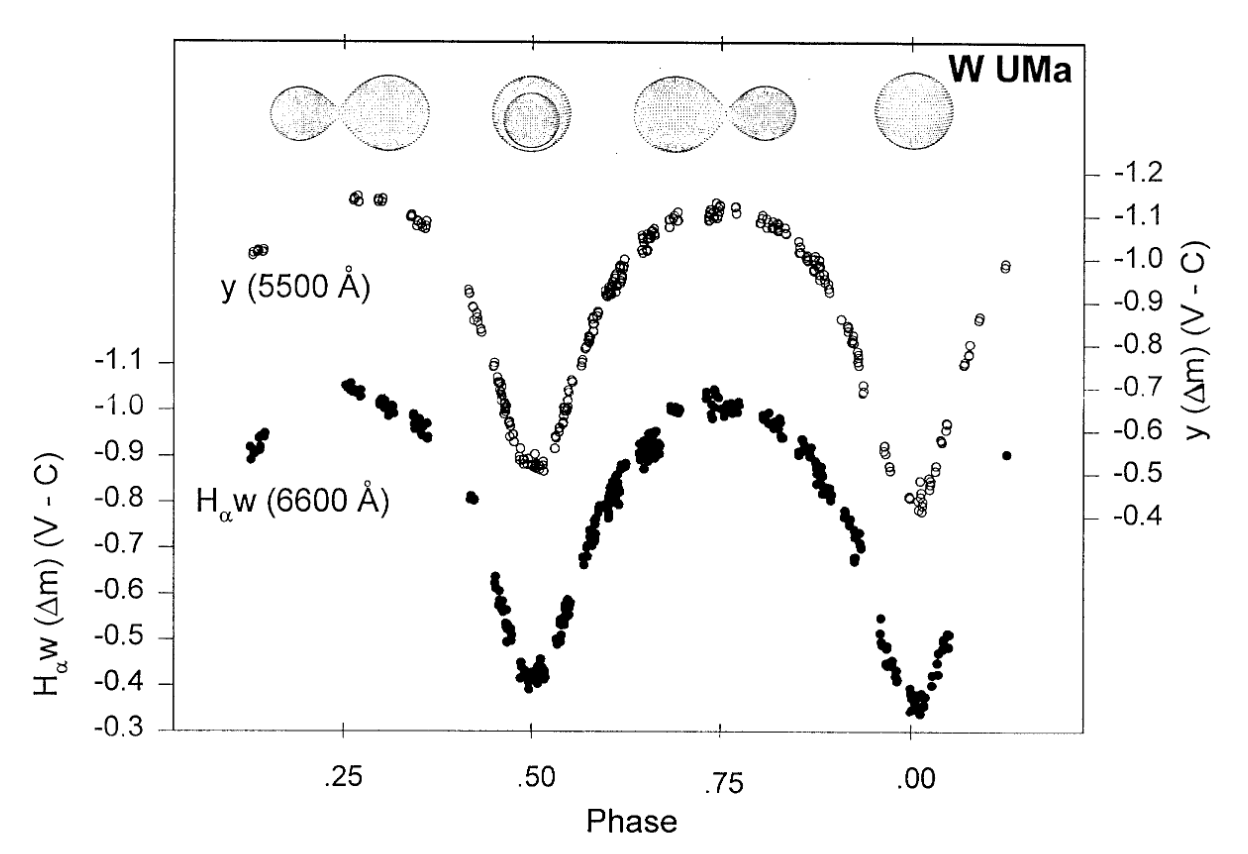
\includegraphics[width= \textwidth]{figs/reused-figs/WUMaLightcurve.png}
            \caption{\textit{This figure shows the light curve of W UMa relative to the apparent position of the system. Reprint from~\parencite{Morgan_1997}}}
            \label{WUMaLightcruve}
        \end{figure}

        % \subsubsection{Simulated}
        % Simulated data is good because of xyz and is useful because of xyz. data was made using xyz

    \subsection{POSYDON Simulations}
        In corroboration with three observed systems I used data generated from the population syntheses tool POSYDON \parencite{Fragos_2023}. I used POSYDON because catalogues of HMXBS and LMXBs are not large enough to fully understand the evolution of these systems. POSYDON is developed and maintained by a team of astrophysicists and computer scientists working at the Université de Genève and Northwestern University. POSYDON uses an additional script called MESA, which is dedicated to single star and binary evolution. POSYDON utilities MESA on a much larger scale in order to simulate full populations. The dataset I used was simulated on the NU super computing Cluster, QUEST. This data was stored in the form of a \.h5 file, containing a total of 6,128,390 rows and 83 columns. (See greatly reduced example of the data frame in table~\ref{POSYDONDataExample} and an HR Diagram of the full dataset in fig.~\ref{EntireDataSetHR})

         \begin{table}[H]
            \centering\
            \footnotesize
            \begin{tabularx}{\textwidth}{||X | X | X | X | X | X | X | X ||}
                \hline 
                \textbf{Binary ID} & 
                \textbf{System State} & 
                \textbf{Orbital Period (days)} & 
                \boldmath$\log_{10}$ \textbf{Mass Transfer Rate} & 
                \textbf{Donor State} & 
                \textbf{Donor Mass} $M_\odot$ & 
                \textbf{Accretor State} & 
                \textbf{Accretor Mass} $M_\odot$
                \\ \hline \hline
                $54$ & Detached & $0.047520$ & $-99.000$ & NS & $1.196033$ & stripped He Core He burning & $\approx 1.002$ \\
                \hline
                $183$ & Detached & $0.0429883$ & $ \approx -80.8$ & NS & $1.196033$ & stripped He Core He burning & $\approx .9957$ \\
                \hline
            \end{tabularx}
            \caption{Example of POSYDON data, heavily modified for readability}
            \label{POSYDONDataExample}
        \end{table}

        \begin{figure}[H]
            \centering
            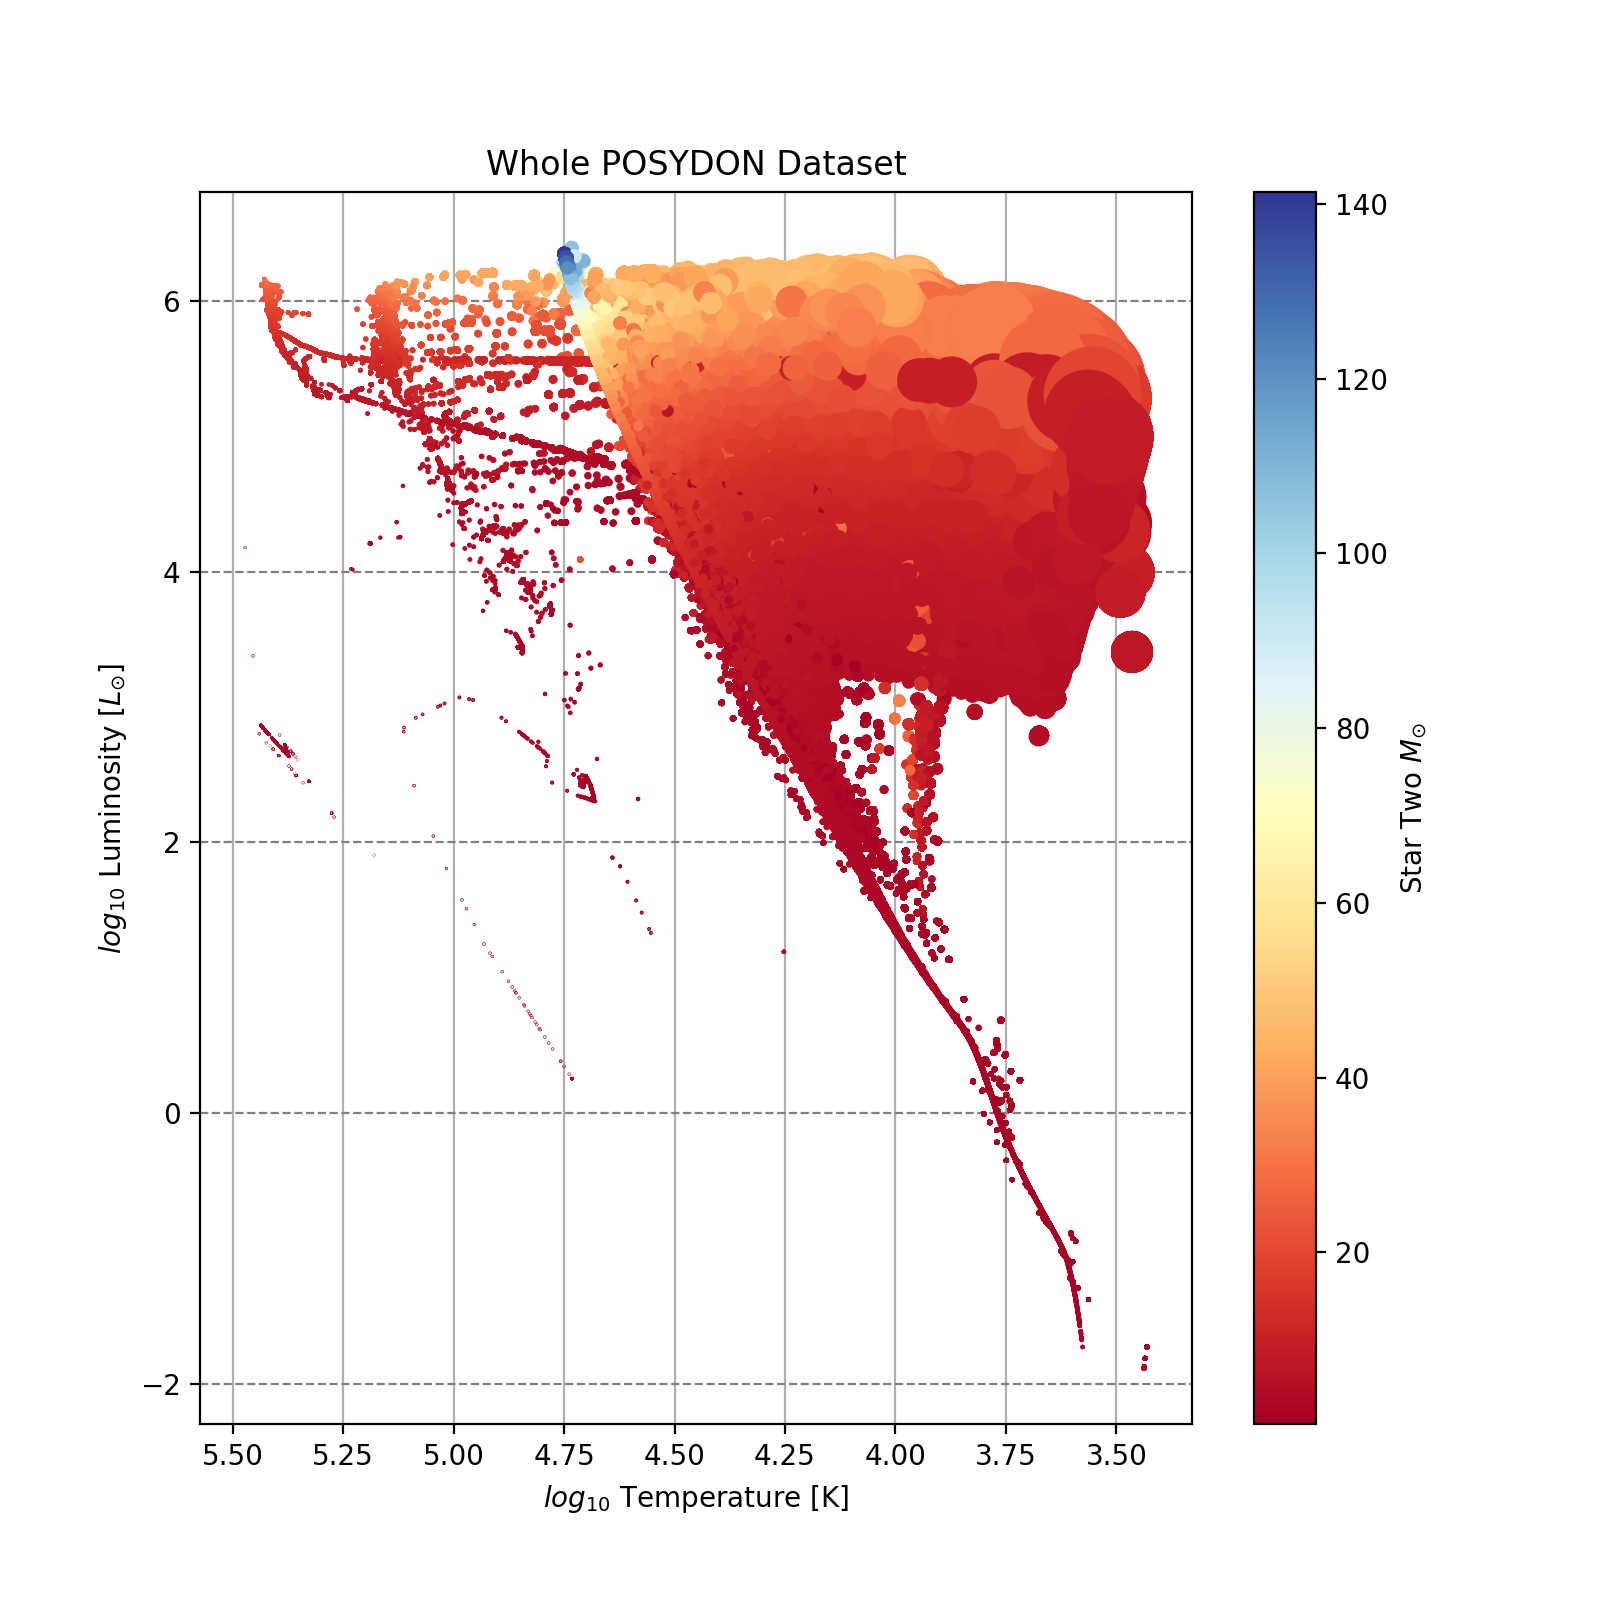
\includegraphics[width = .7\textwidth]{figs/GeneratedFigs/WholePOSYDONDatasetExample.png}
            \caption{HR Diagram of the donor star for the full POSYDON dataset ($\approx$6.1 million points). This shows the stars evolutionary tracks over the span of 13.8 billion years. Note that the color of the plotted points correspond to the solar mass of the donor star. Additionally, the radius of each plotted point corresponds with the radius of the simulated star. Generated with Matplotlib~\parencite{Matplotlib}.}
            \label{EntireDataSetHR}
        \end{figure}


        This dataset looks very similar to a standard HR diagram, however, there are some key population differences. In the center we can see the Main sequence
        \subsubsection{Data Processing}
            With my research I sought to contextualize these very specific systems, allowing one to better understand how these systems play into the larger picture of binaries. In order to do this I utilized a large dataset generated from POSYDON. In order to properly analyze this data I utilized Python with a large quantity of packages. These packages included Pandas \parencite{reback2020pandas}, Matplotlib \parencite{Matplotlib}, and NumPy \parencite{harris2020array}. These tools allowed me to rapidly and efficiently analyze the large amount of data, something this paper would not have been possible without.  As I analyzed the data, I found there were certain processes regarding data processing and graphing that I was doing repeatedly, so I wrote a custom Python script in order to streamline the process. This script allowed quickly generate variable HR diagrams for any and all types of datasets, quickly adjusting variables as needed while automatically applying them to all the curated graphs. This script can be found on the GitHub page for the paper at \url{https://github.com/PiersonLip/Honors-Independent-Study/blob/main/Code/HRDiagram.py}.

            I worked on this entirely in VS Code, as it provided a great environment for me to work efficiently and worked very well with \LaTeX. I utilized Python notebook files in order to analyze the data at greater speed.


\section{Results}
    I found a lot of the key factors in mass transfer and how it affected various types of binary stars, with Full-blown RLO being the most key factor in mass transfer in low-mass x-ray binaries, leading to large amounts of x-ray emission (sect.~\ref{XrayAccretion}). This process had drastic effects on both the donor and accretor star.

    I found that a large quantity of detached systems will experience mass transfer in some form. This mass transfer is in the form of wind accretion or atmospheric Roche Lobe Overflow (sect.~\ref{WindAccretion}).

    I found that mass can will be transferred between stars in contact binaries, with a majority of contact binaries not actually being stable, but instead in a phase of their life called common envelope (sect.~\ref{CommonEnvelope}).
    
    I found that V404 Cyngi properties did not fall onto a known location on an HR Diagram (fig.~\ref{V404FullContextTesting}). This suggests that either the simulated data generated using POSYDON has an error, or that the observed data is incorrect. It is much more likely that there is a fault with POSYDON (or even MESA itself) when it comes to simulating LMXBs. This could pose a larger issue, as a lot of papers utilize POSYDON and/or MESA to come to their conclusions. 
        
        \subsection{Detached Binaries}`'\label{sect:detachedResults}
            Despite the nature of detached systems they are still able to transfer mass a number of ways \parencite{TaurisvandenHeuvel+2023}. A large quantity of these systems are classified as HMXBs due to wind accretion (sect.~\ref{WindAccretion}), where a star of great enough mass is able to transfer some of that mass through stellar winds \parencite{TaurisvandenHeuvel+2023}. However, these systems, despite being technically detached, are close to filling their RL (sect.~\ref{RLModel}). Because of this, it is not unheard of for them to also transfer mass through full-blown RLO (sect.~\ref{RLO}) \parencite{TaurisvandenHeuvel+2023}. Additionally, their atmosphere can be transferred through RLO while their mass itself is not, in which case it is called atmospheric RLO (sect.~\ref{atmosphericRLO}). 

            
        \begin{figure}[H] 
            \centering
            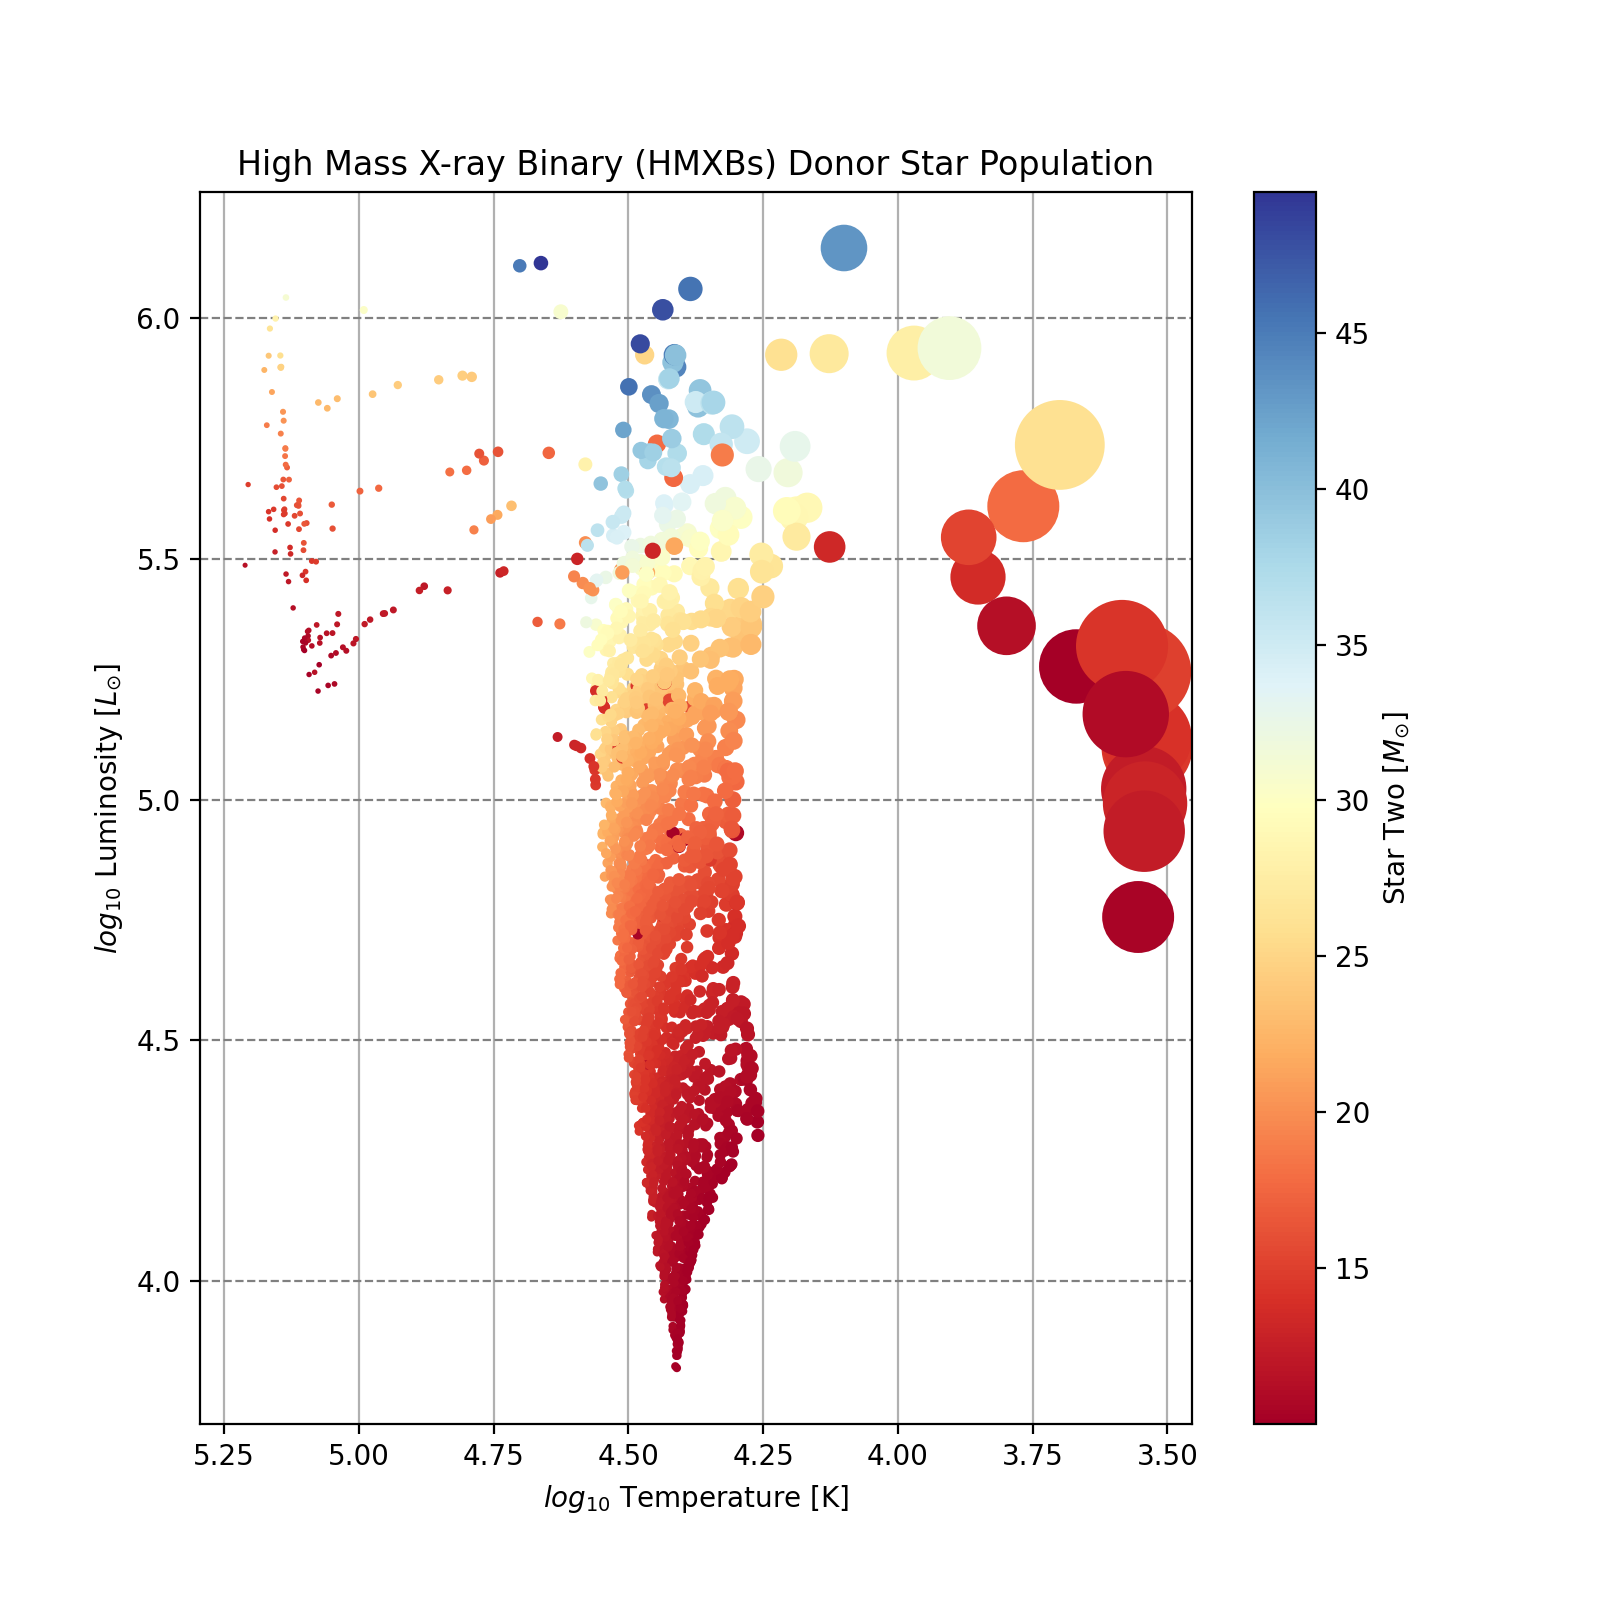
\includegraphics[width=.7\textwidth]{figs/GeneratedFigs/VelaX-1/HMXBHRPopulation.png}
            \caption{HR Diagram of HMXBs using POSYDON generated data. The size of the plotted dot corresponds to the size of the star.}
            \label{HMXBsHRDiagram}
        \end{figure}

        \begin{figure}[H] 
            \centering
            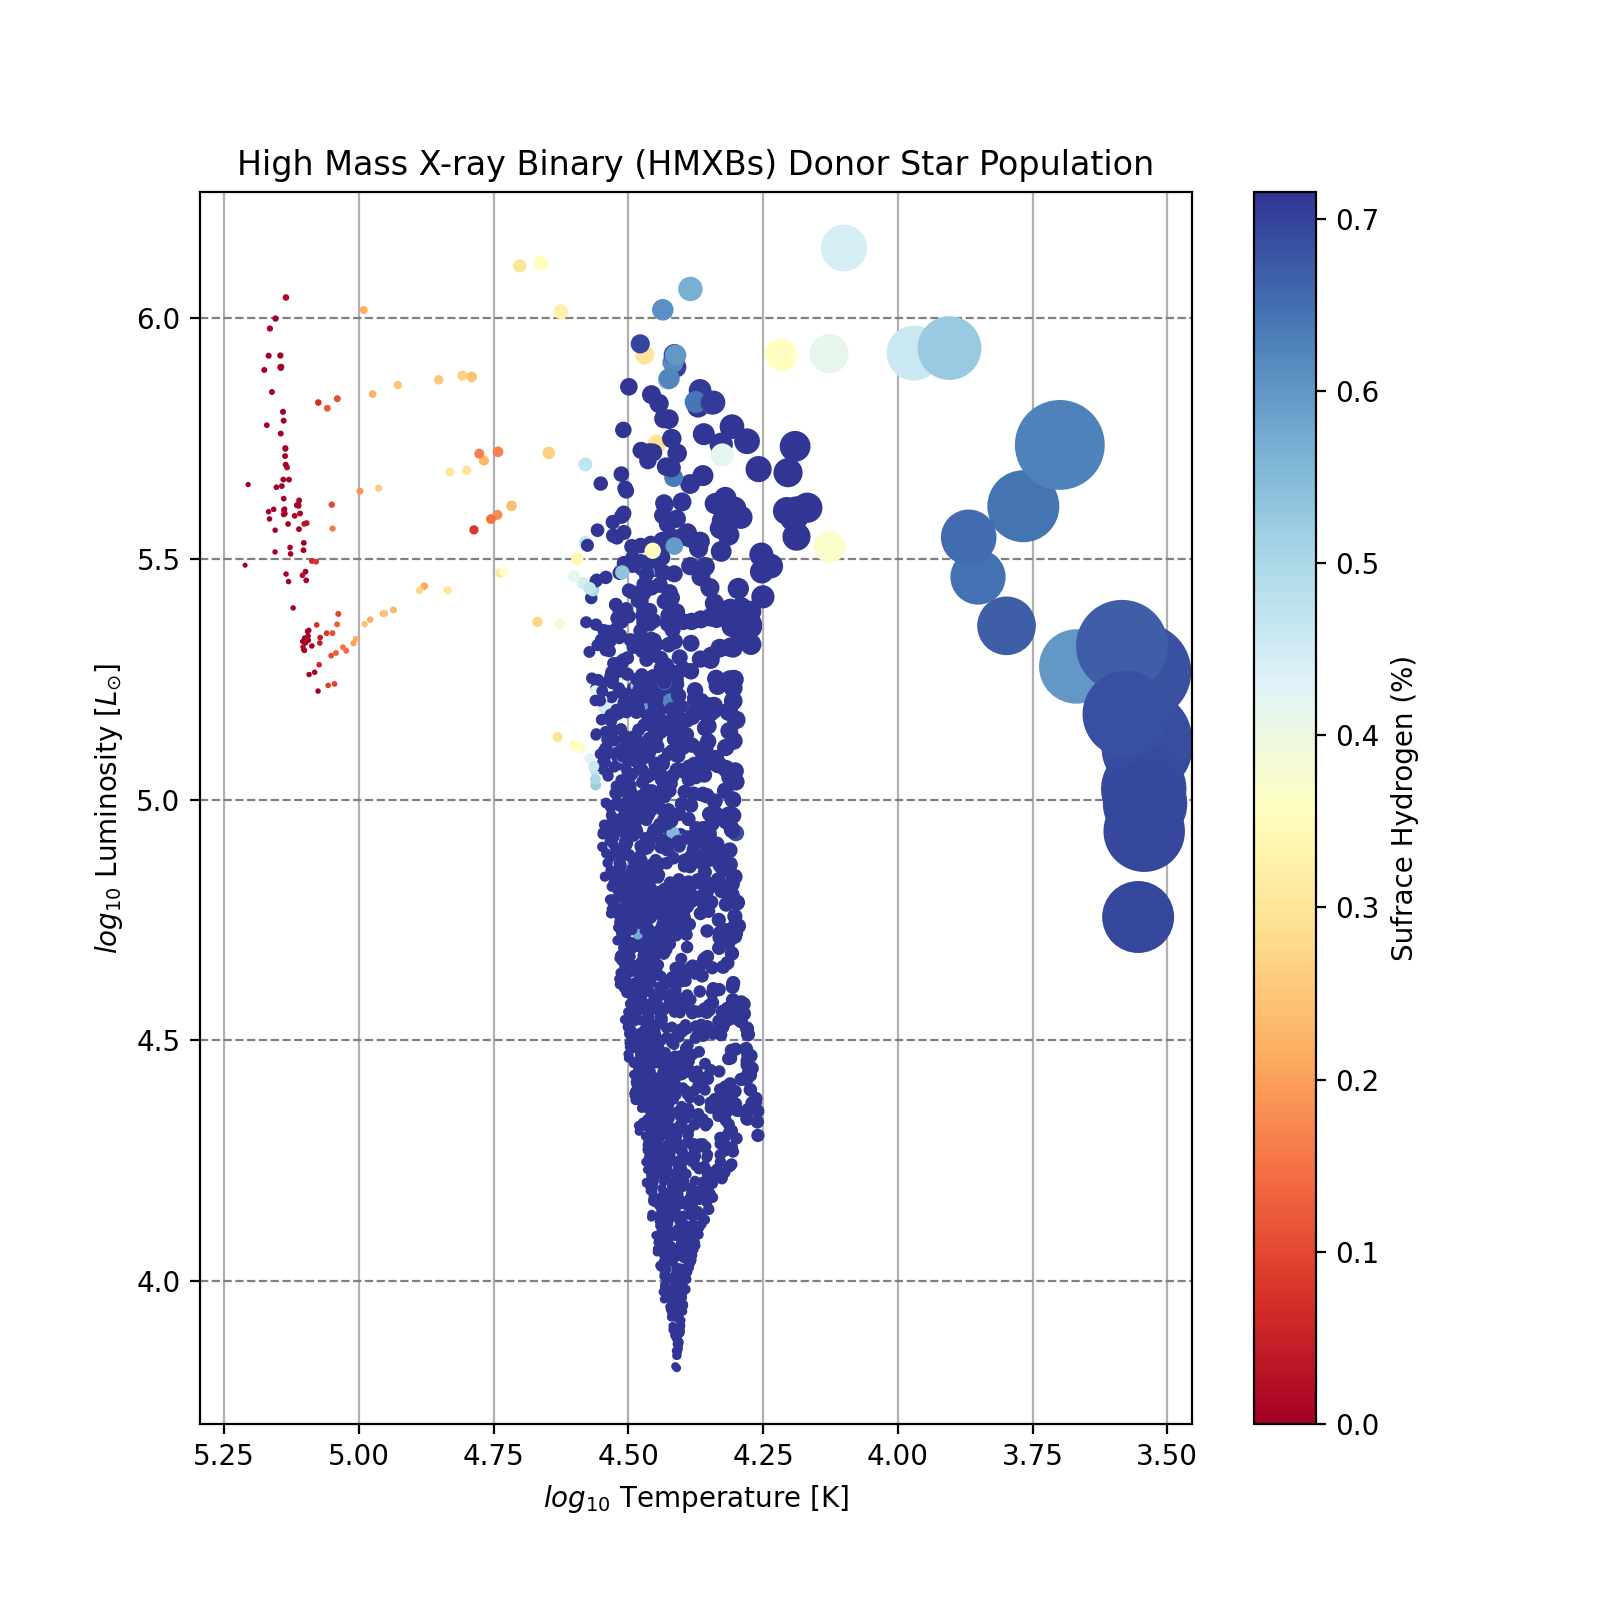
\includegraphics[width=\textwidth]{figs/GeneratedFigs/VelaX-1/HMXBsSurfaceCompHRDiagram.png}
            \caption{HR Diagram of HMXBs using POSYDON generated data. The color the star corresponds to the percentage amount of surface hydrogen.}
            \label{HMXBsSurfaceCompHRDiagram}
        \end{figure}

        In figure~\ref{HMXBsHRDiagram} we can see that while the majority of the donor stars in HMXBs are main sequence, a large quantity of them are also Wolf-Rayet type (see fig.~\ref{HMXBsSurfaceCompHRDiagram}) and supergiants (see size of the stars in fig.~\ref{HMXBsHRDiagram}). This is to be expected due to the high masses of the donor star population.  

            \subsubsection{Vela X-1 Results} \label{VelaX1Results}

            In figures~\ref{VelaX1XrBPopulationHRComp} and~\ref{VelaX1HMXBPopulationHRComp} we see that Vela X-1 is one of the more extreme example of HMXBs, as it has a higher temperature and luminosity then a lot of its similar stars, the majority of which are in main sequence. Additionally, we can also confirm the fact that Vela X-1 is a giant star due to its location and proximity to other giants on the HR Diagram (fig.~\ref{VelaX1HMXBPopulationHRComp}), something which is corroborated by \parencite{Kretschmar_2021}.

            \begin{figure}[H] 
                \centering
                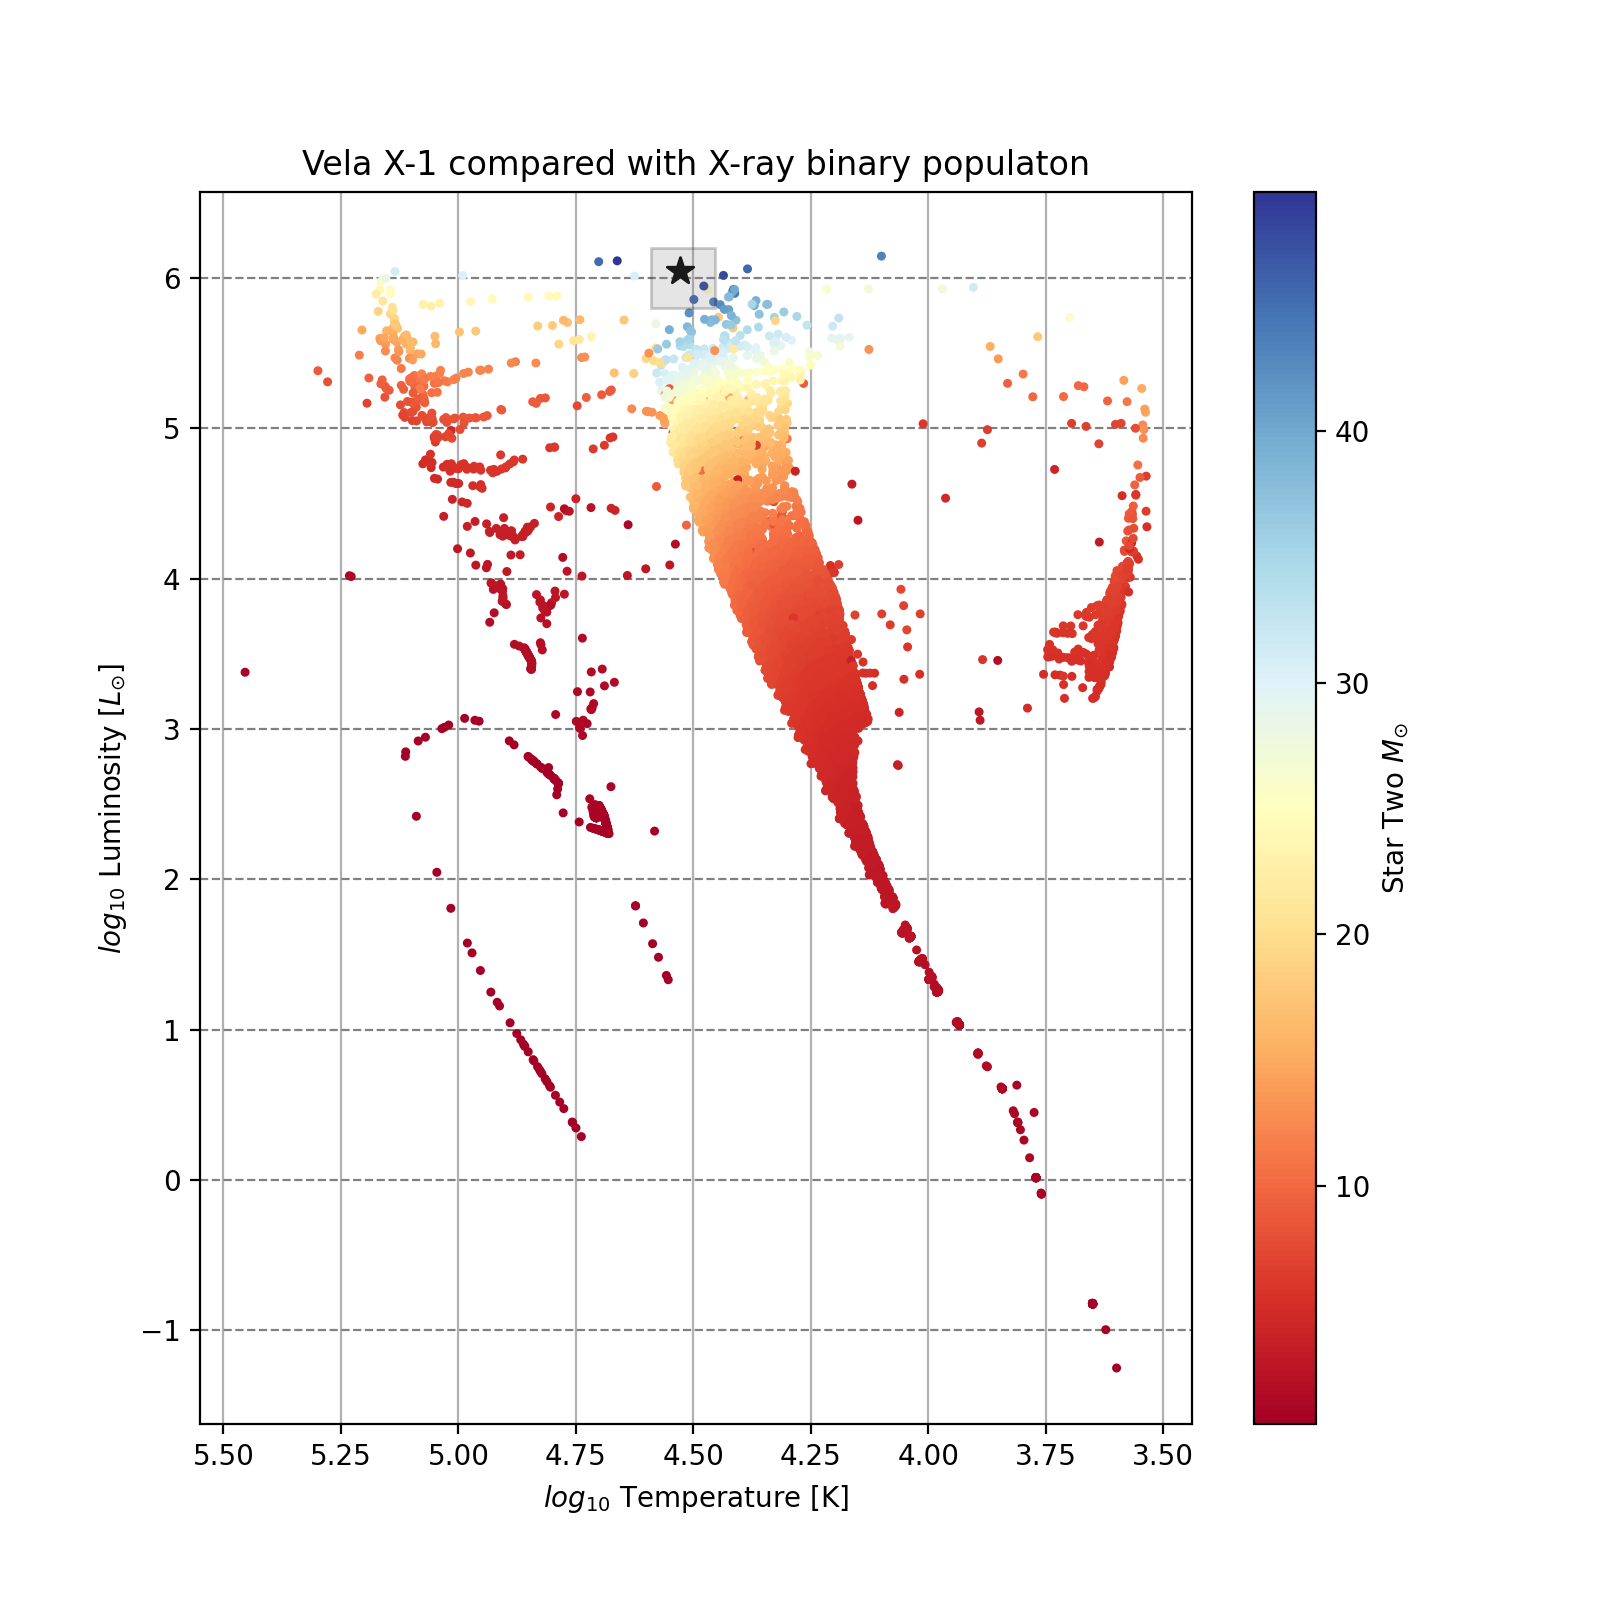
\includegraphics[width=\textwidth]{figs/GeneratedFigs/VelaX-1/VelaX1XrBPopulationHRComp.png}
                \caption{HR Diagram with reference for Vela X-1. The star is the mean value of observation range, box is overlap of the min and max temperature and luminosity values.}
                \label{VelaX1XrBPopulationHRComp}
            \end{figure}

            \begin{figure}[H] 
                \centering
                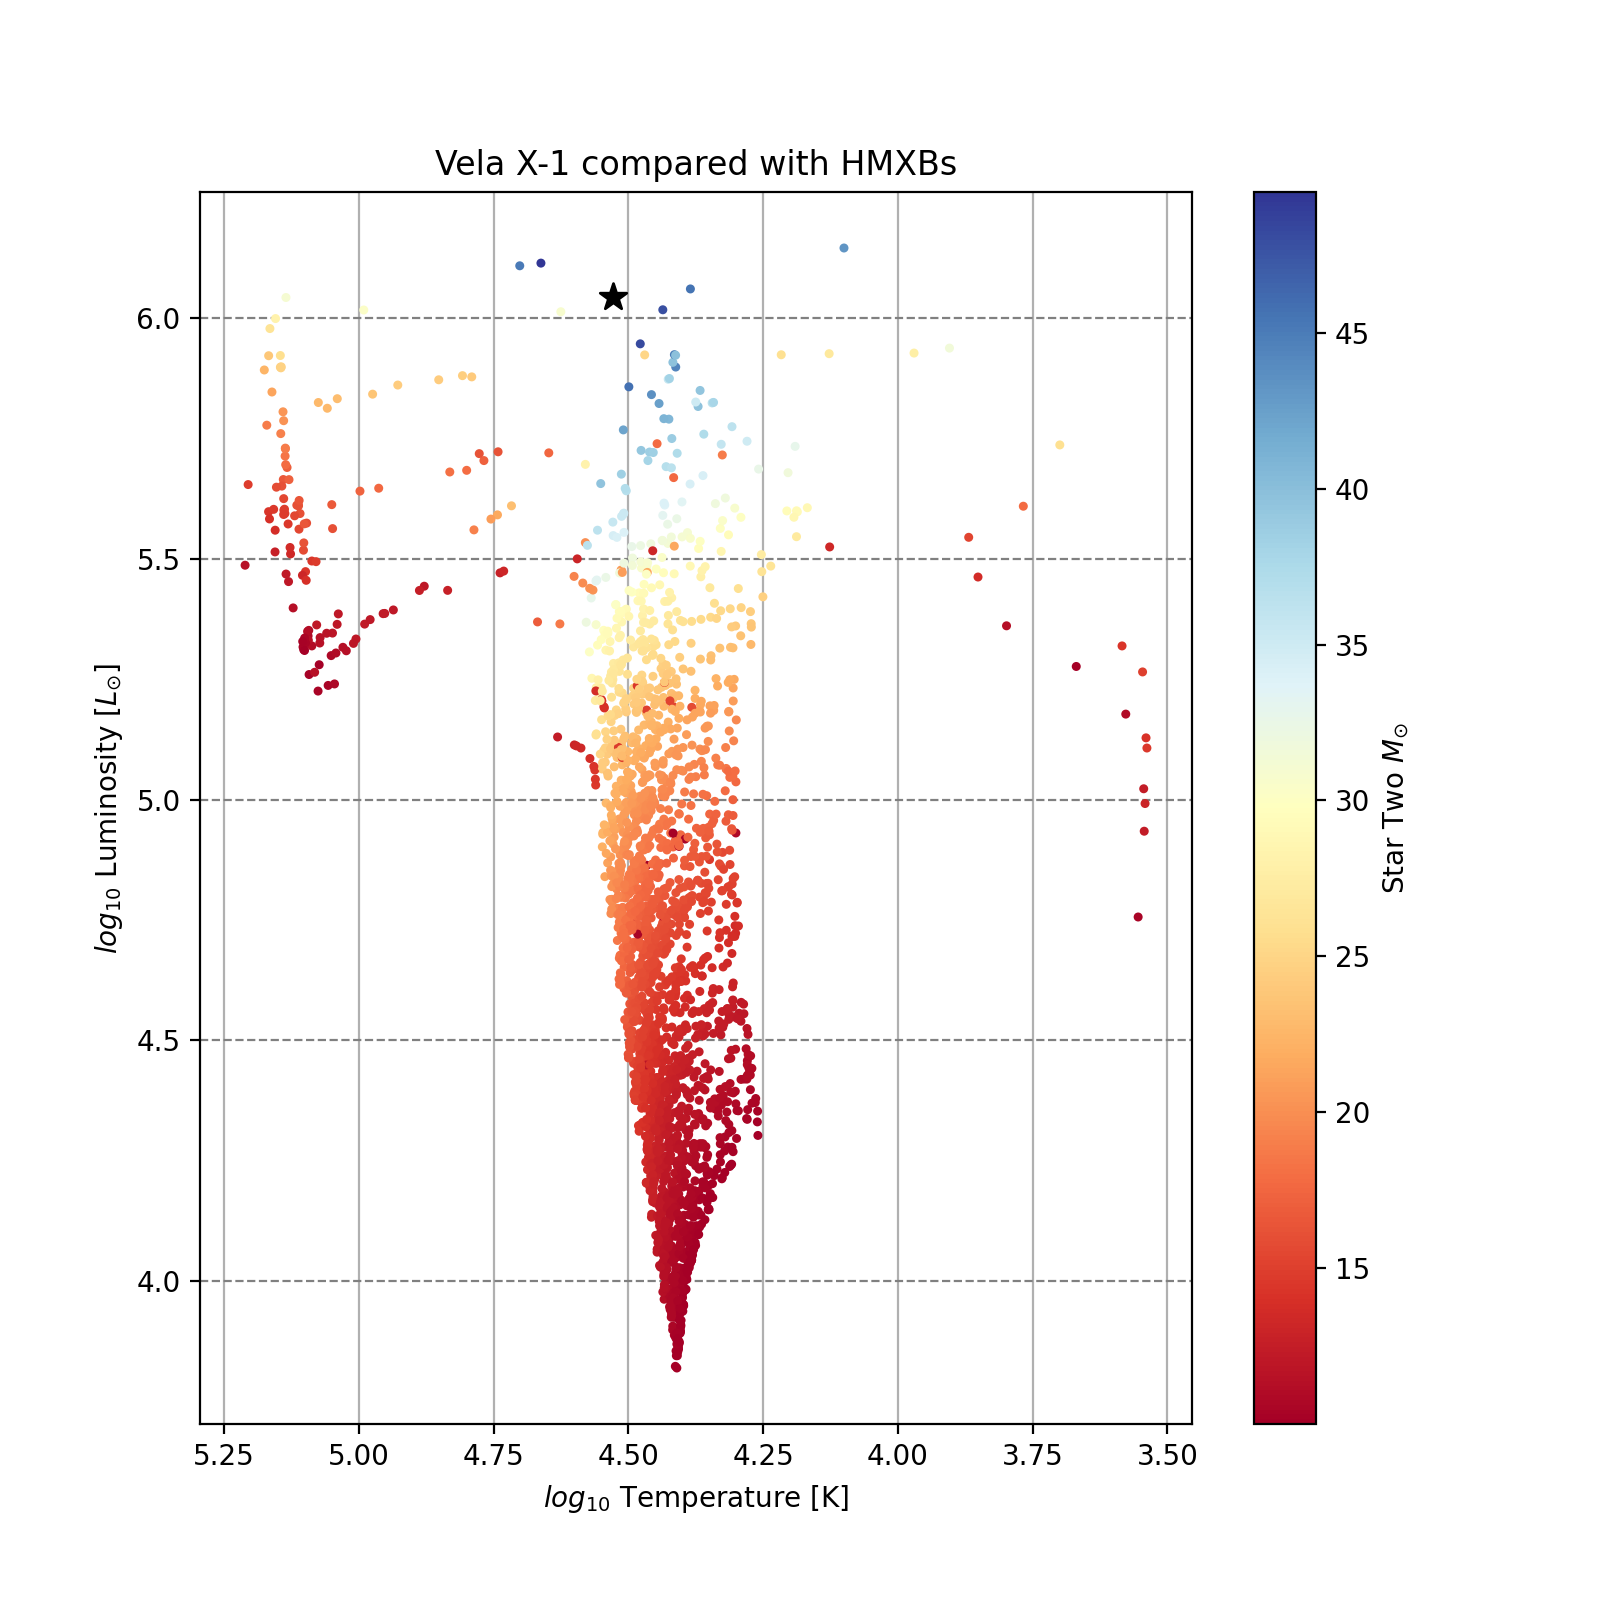
\includegraphics[width=\textwidth]{figs/GeneratedFigs/VelaX-1/VelaX1HMXBPopulationHRComp.png}
                \caption{HR Diagram of HMXBs with reference point for Vela X-1. The star is the mean value of observation range, box is overlap of the min and max temperature and luminosity values.}
                \label{VelaX1HMXBPopulationHRComp}
            \end{figure}
    
    % This is particularly interesting as Vela X-1s luminosity and temperature would make it a likely candidate to be a Wolf-Rayet star,

    
    \subsection{Semi-Detached Binaries} \label{sec:SemiDetachedResults}
        \begin{figure}[H]
            \centering
            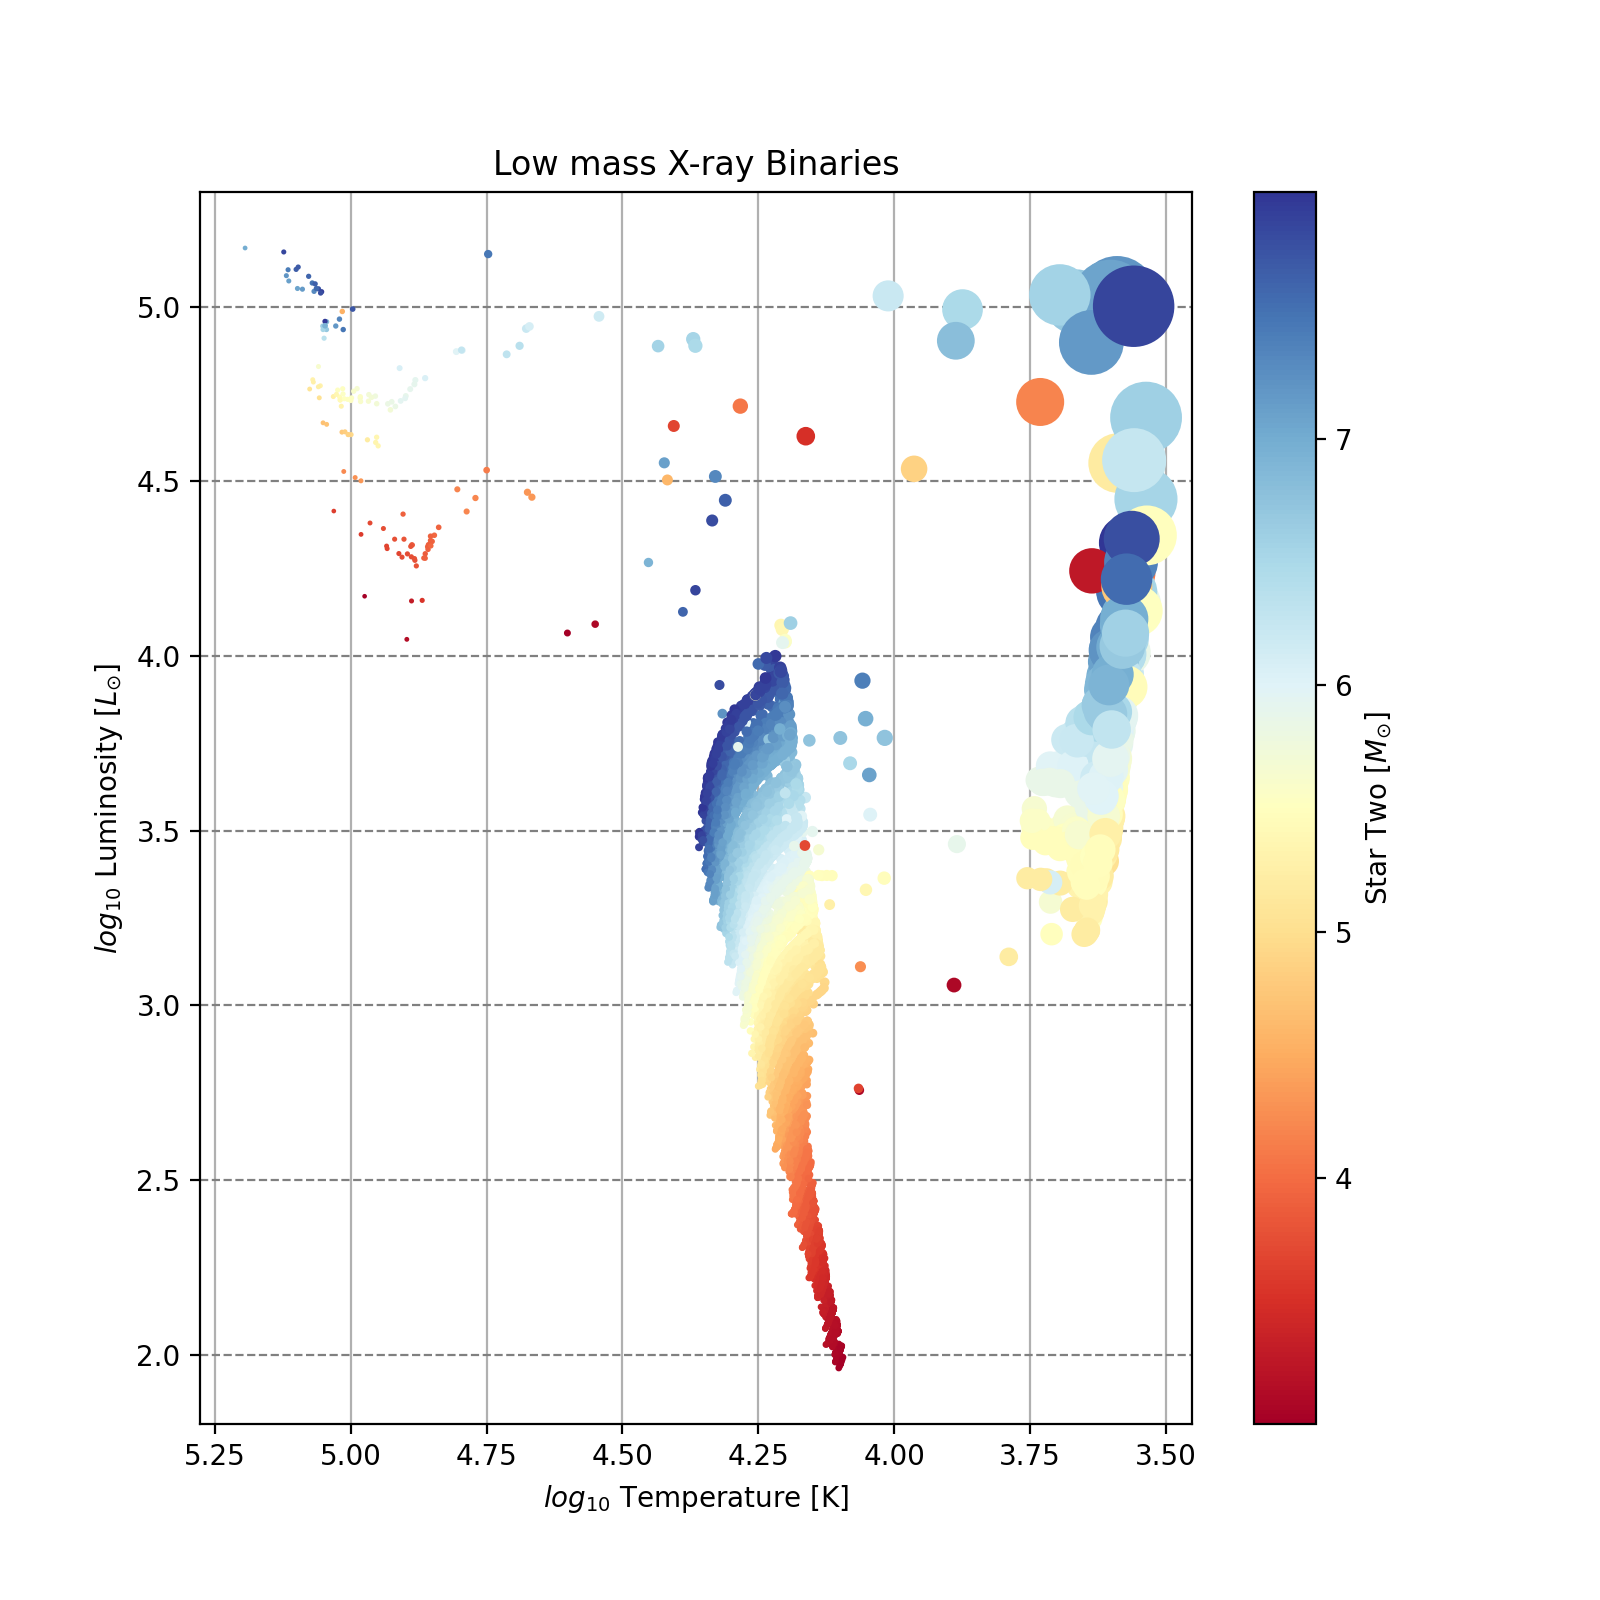
\includegraphics[scale = .6]{figs/GeneratedFigs/V404_Cygni/LMXBsHRDiagram.png}
            \caption{HR diagram of the donor star in Low mass X-ray Binaries. Size of the plotted dot corresponds to the size of the star.}
            \label{XrayBinaryHRDiagram}
        \end{figure}
       RLO a very common phenomena in binary star evolution, with the majority of systems undergoing it as an evolutionary phase during their lifetime \parencite{TaurisvandenHeuvel+2023}. RLO is most commonly and directly observed in LMXBs \parencite{TaurisvandenHeuvel+2023}, as these systems can allow for a stable transfer of mass from a donor to an accretor, which can create emission of x-rays \parencite{TaurisvandenHeuvel+2023} (sect.~\ref{XrayAccretion}). Furthermore, RLO can either be stable or unstable with that most important factors in stability being the mass ratio of the stars, the eccentricity of the system, and the stars' envelope type (sect.~\ref{RLO}). This mass is transferred through the Lagrange point $L_1$ due to a pressure differential \parencite{TaurisvandenHeuvel+2023} (sect.~\ref{L1MassTransfer}). 

        In figure~\ref{XrayBinaryHRDiagram} we can see that X-ray binaries' donor stars generally follow a semi-standard HR diagram with the location of the stars being congruent with what we would expect of lower mass donor stars. This is evident in selection of the main sequence branch we see, as there is a distinct cut-off point.

        \subsubsection{V404 Cygni Results}~\label{V404Results}
            \begin{figure}[H] 
                \centering
                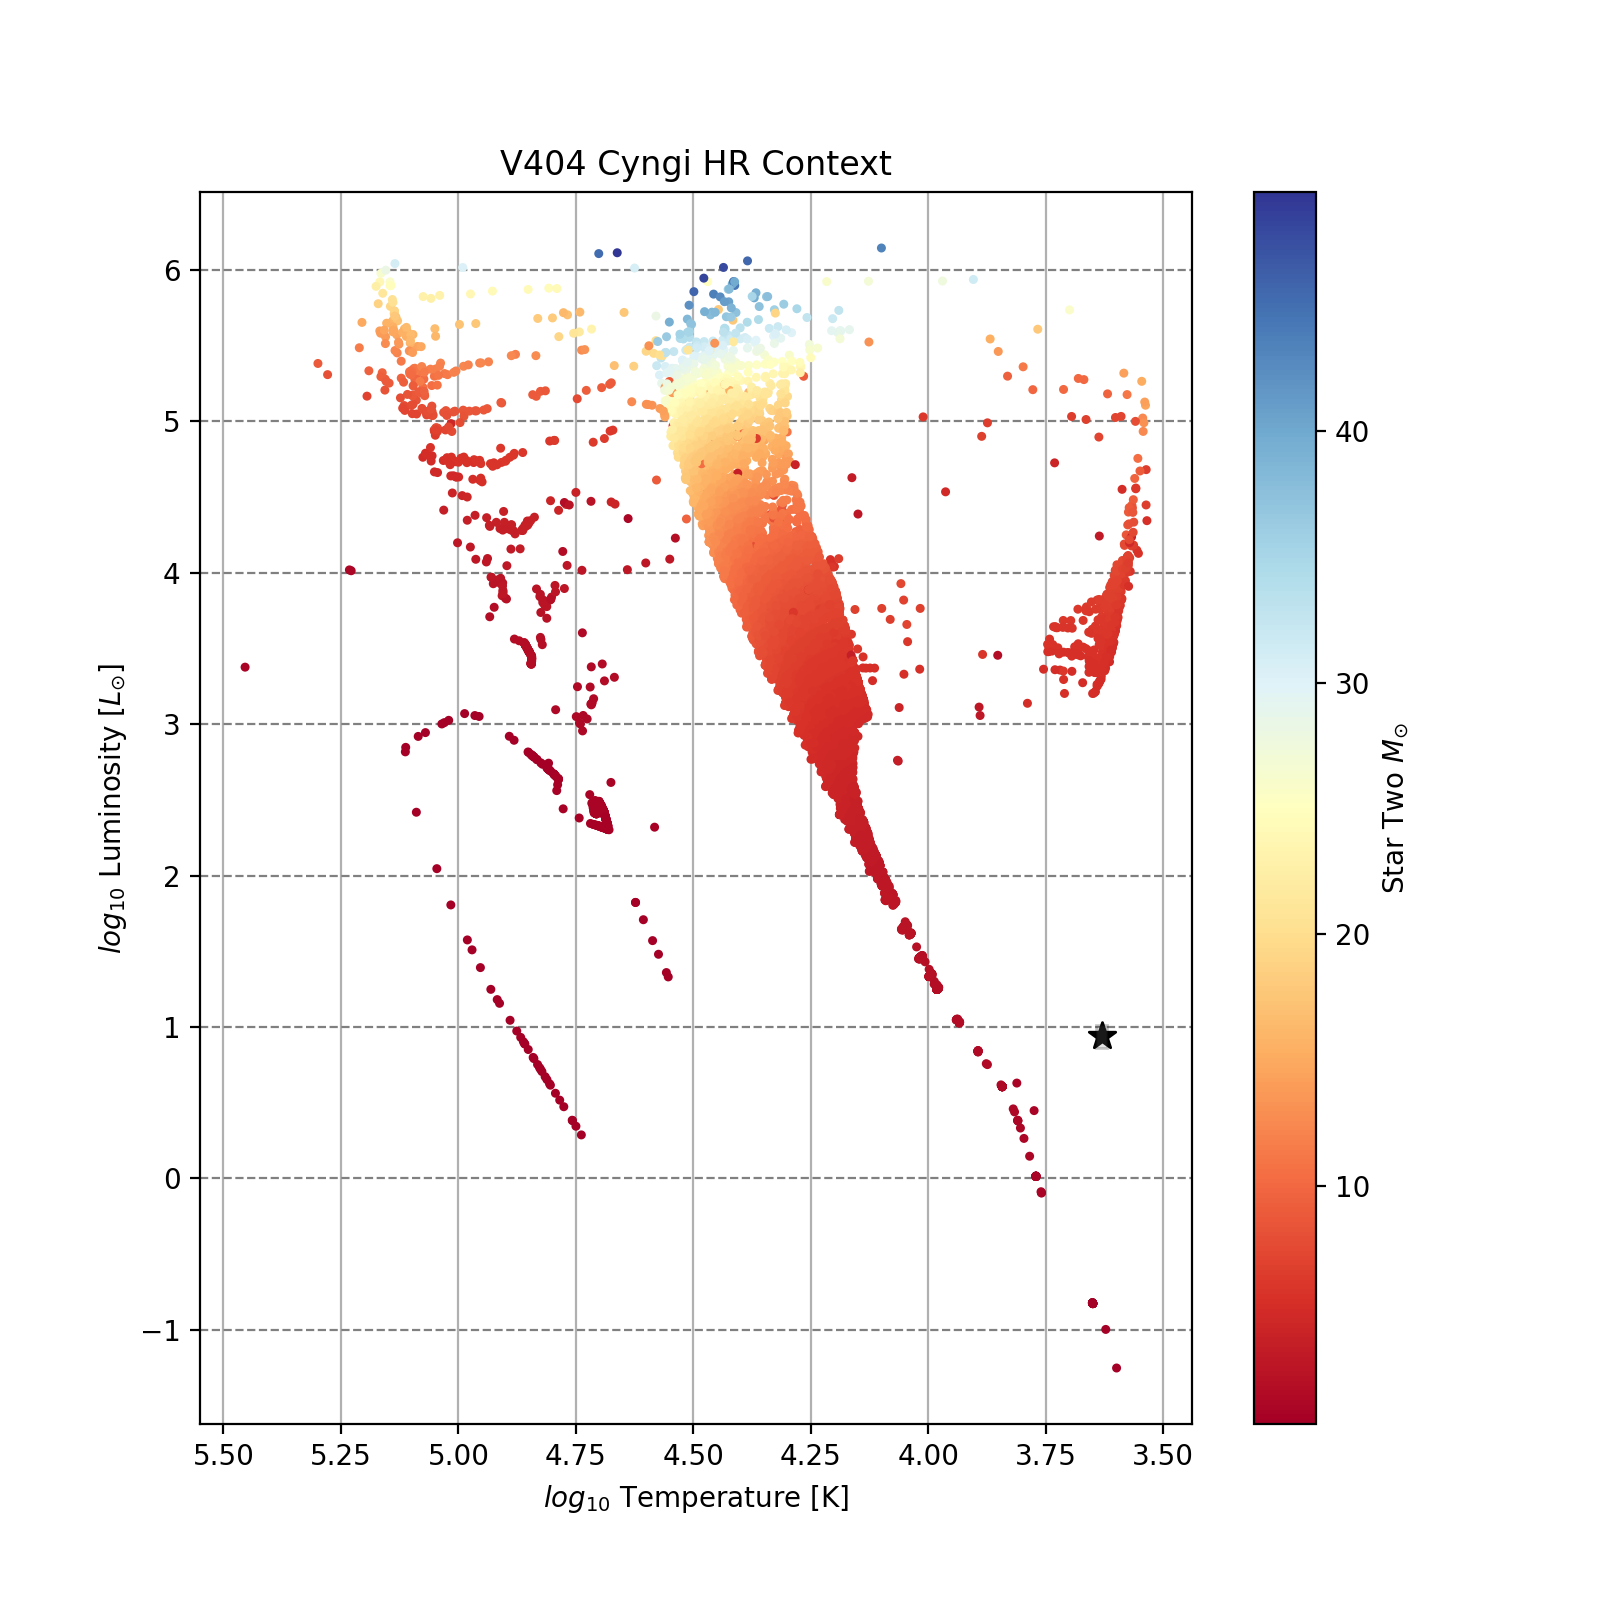
\includegraphics[scale = .6]{figs/GeneratedFigs/V404_Cygni/V404XBsPopulationHRComp.png}
                \caption{HR Diagram with reference for V404 Cygni. Utilizing data from \parencite{Bartolomeo_2023}. Note that the range of error \textit{is} plotted, however, does not play an effect on the location of the star}
                \label{V404Context}
            \end{figure}

            V404 Cygni does not fall onto the two main simulated evolutionary tracks for LMXBs. This distinct discontinuity between the observed temperature and luminosity and expected location on an HR diagram suggests there exists an error. It is more likely that the simulated data possess the error, as V404 Cygni has been observationally measured to high accuracy. I believe this discrepancy comes from V404 Cygnis' unique properties (table~\ref{V404Data}) as it is uncommon for a star to lose such a large amount of mass and be so tightly constrained to its accretor as we see in \parencite{Bartolomeo_2023}. I believe that POSYDON likely did not account for such an extreme case. However, further investigation of both simulated and observed data is needed to get a full conclusion. 

            While investing this I tried a multitude of different things. This included getting more recent data of V404 Cygni from \parencite{Bartolomeo_2023}, graphing an error range around the plotted star (fig.~\ref{V404Context}), and plotting the entire dataset including all the stars evolution over time (fig.~\ref{V404FullContextTesting}). None of these lead to any breakthroughs. 

            \begin{figure}[H] 
                \centering
                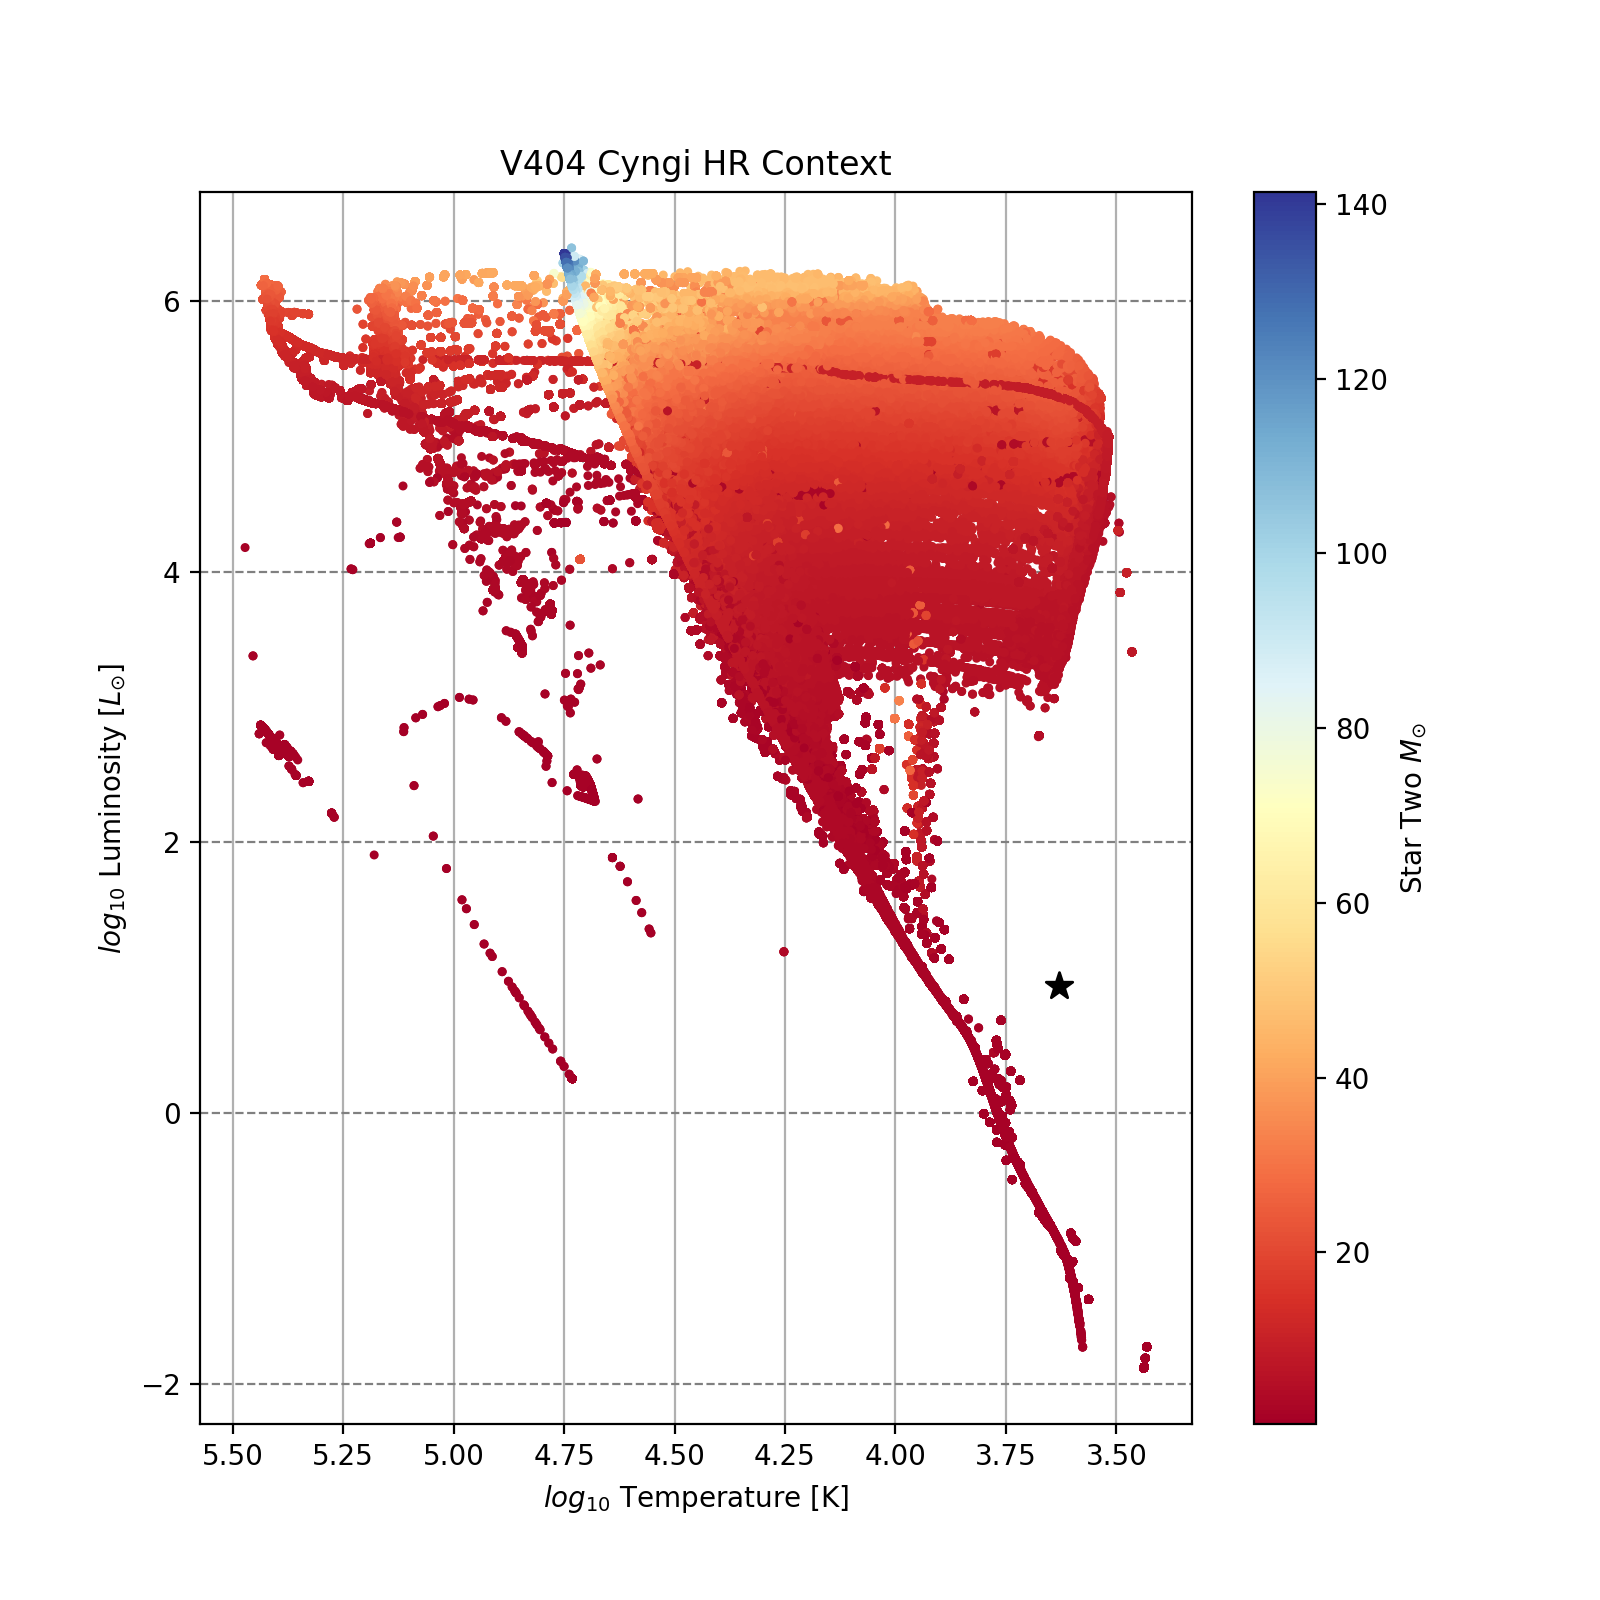
\includegraphics[scale = .6]{figs/GeneratedFigs/V404_Cygni/V404EntireDatasetPopulationHRComp.png}
                \caption{HR Diagram with reference for V404 Cygni. Utilizing data from \parencite{Bartolomeo_2023}. Still off of any plotted evolutionary track despite being plotted with the entire dataset.}
                \label{V404FullContextTesting}
            \end{figure}

        %contact binaries
        \subsection{Contact Binaries}
            Mass transfer in contact binaries happens in a variety of cases. In some systems where both of the stars RL's are full (fig~\ref{ContactBinaryRL}), the system can in a multitude of states. The most prominent of these is common envelope (\ref{CommonEnvelope}) and an actual contact binary. It is important to note that CE is a temporary stage which many different types of binaries evolve through, whereas a contact binary is a population themselves.

            I found that in mass transfer in an evolving contact binary causes a mass oscillation between the two stars \parencite{Fabry_2025} (fig.~\ref{qEvolution}), where the stars will transfer mass back and forth. This process will continue until the mass ratio between the two stars crosses a critical threshold, after which the stars will then merge \parencite{Fabry_2025}. 

        \begin{figure}[H]
            \centering
            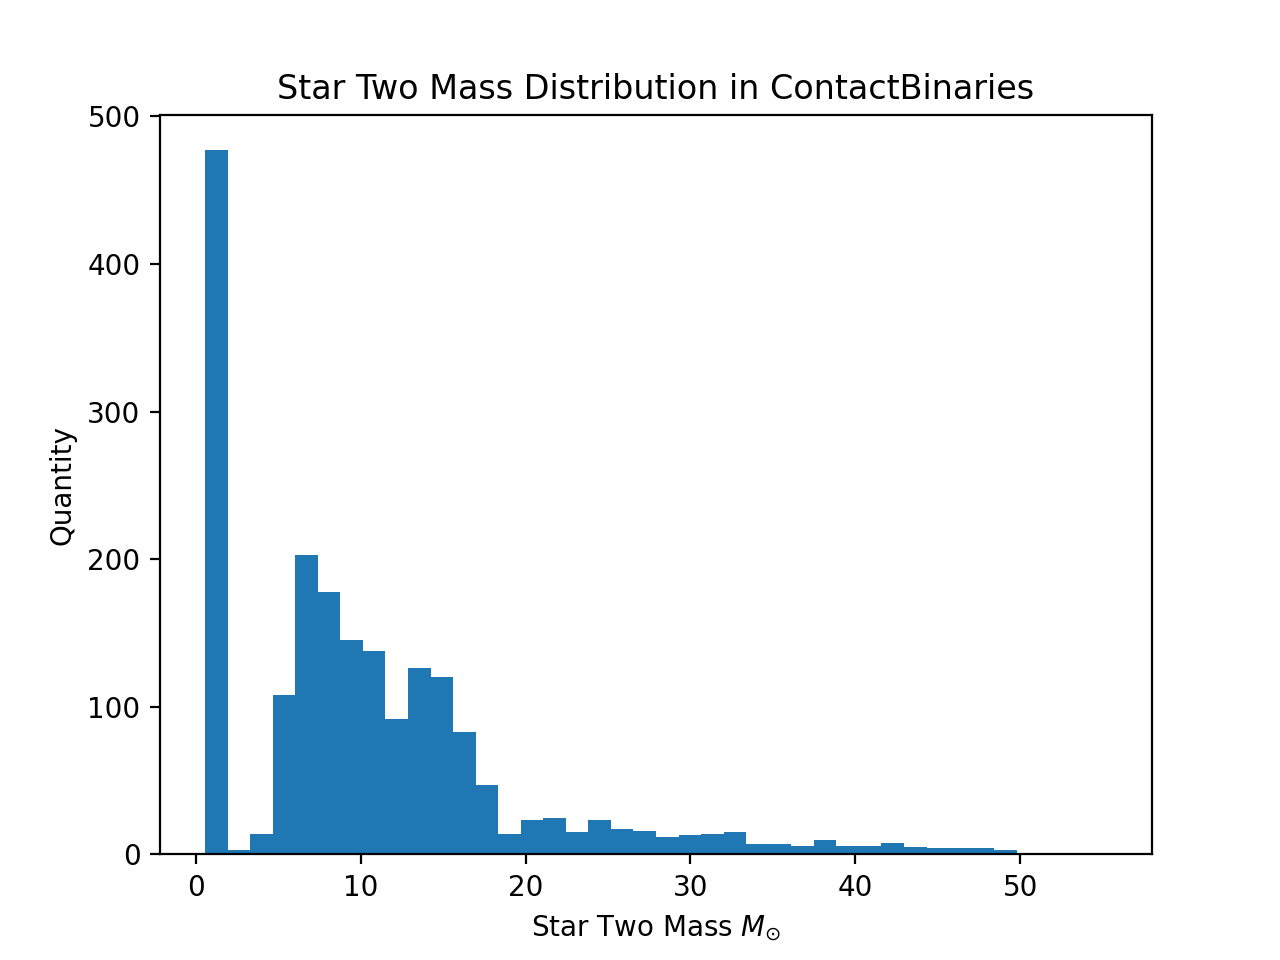
\includegraphics[width = .8\textwidth]{figs/GeneratedFigs/W_UMa/ContactBinaries_Star_Two_Mass_Distribution.png}
            \caption{Star two mass distribution for contact binaries}
            \label{contactBinaryStar2MassDistro}
        \end{figure}

        In figure~\ref{contactBinaryStar2MassDistro} we can see that contact binaries mass distribution feature a prominent spike at around one solar mass, with a distribution centered around 10, and then a scattered amount afterward. 

        \begin{figure}[H]
            \centering
            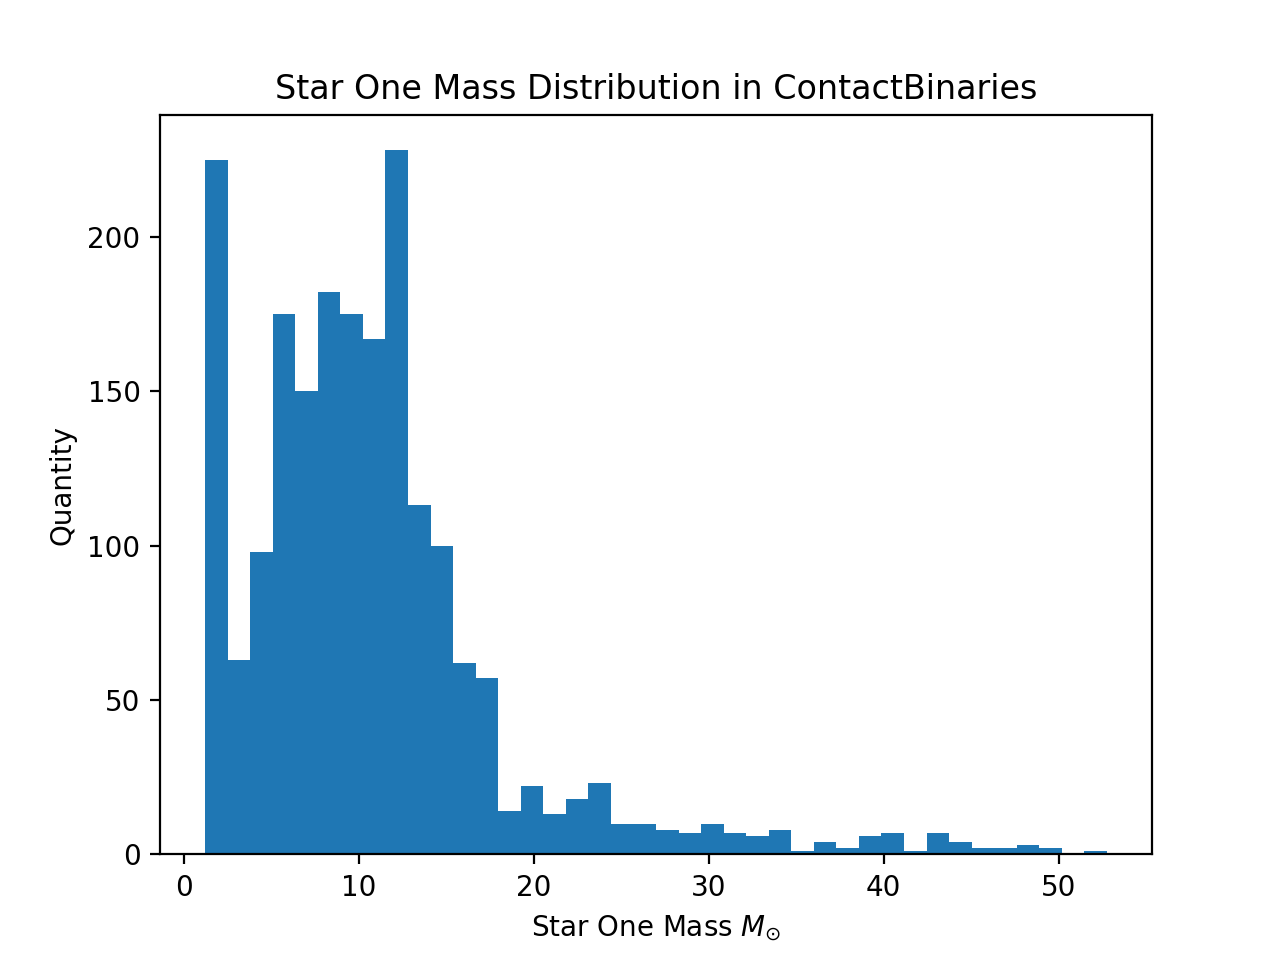
\includegraphics[width = .8\textwidth]{figs/GeneratedFigs/W_UMa/ContactBinaries_Star_One_Mass_Distribution.png}
            \caption{Star one mass distribution of contact binaries}
            \label{contactBinarStar1MassDistro}
        \end{figure}

        Note how similar this is to the star two distribution. From the POSYDON data, I found the mean mass of star one in contact binaries to be $\approx 10.703$ and star two to be $\approx 10.6548$. This is congruent with what previous papers have found \parencite{Fabry_2025}. This is due to the nature of mass transfer in contact binaries leading to an equalization in masses. As a contact system evolves, the mass transfer causes q (the mass ratio between stars) to stabilize to a value of $q\approx1$ \parencite{Fabry_2025}. We can clearly see this oscillation and then stabilization in figure~\ref{qEvolution}. The cause of the difference in fig.~\ref{contactBinaryStar2MassDistro} and~\ref{contactBinarStar1MassDistro} is because of the nature of the simulated data, as the initial grid was predisposed for star one binary to have a greater mass in order to increase the likelihood of mass transfer. 

        \begin{figure}[H]
            \centering
            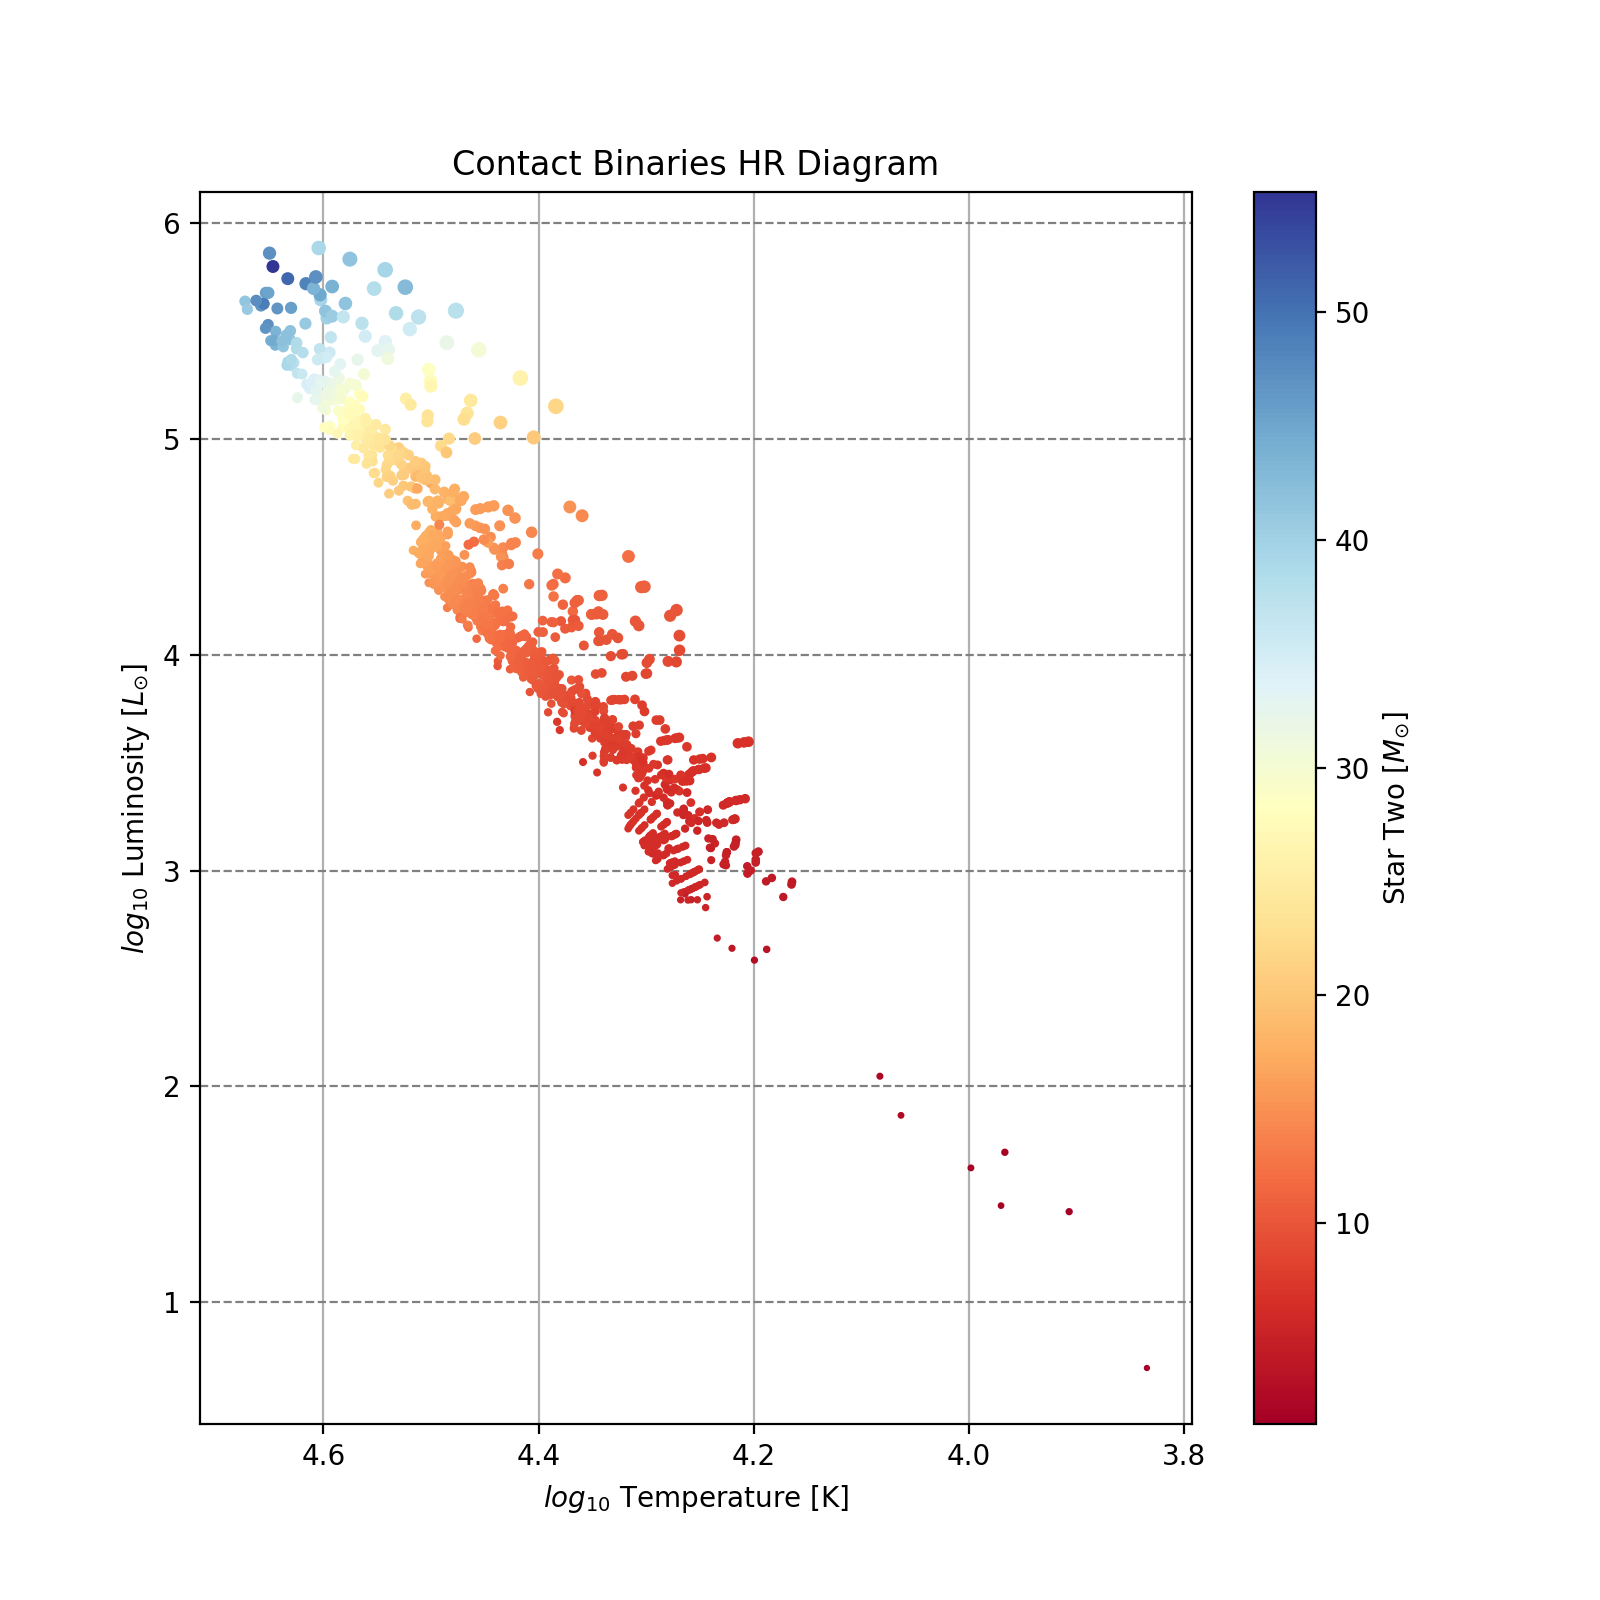
\includegraphics[scale = .6]{figs/GeneratedFigs/W_UMa/ContactbinaryHRDiagram.png}
            \caption{HR diagram of contact binaries from POSYDON data, generated with Matplotlib.}
            \label{contactBinaryHRDiagram}
        \end{figure}

        This is one of the more interesting results, as we can see that contact binaries form a very specific population on the HR diagram, falling on specific linear with a linear relationship (fig.~\ref{contactBinaryHRDiagram}) I believe this is because of the stabilizing natures regarding mass ratios in contact binaries. However, this requires further investigation before anything conclusions can be formed as there are many other reasons relationship could emerge. Other causes include the inherent skewing of the grid, observation bias and known simulation error. 
        
        \subsubsection{W UMa Cygni Results}
            \begin{figure}[H]
                \centering
                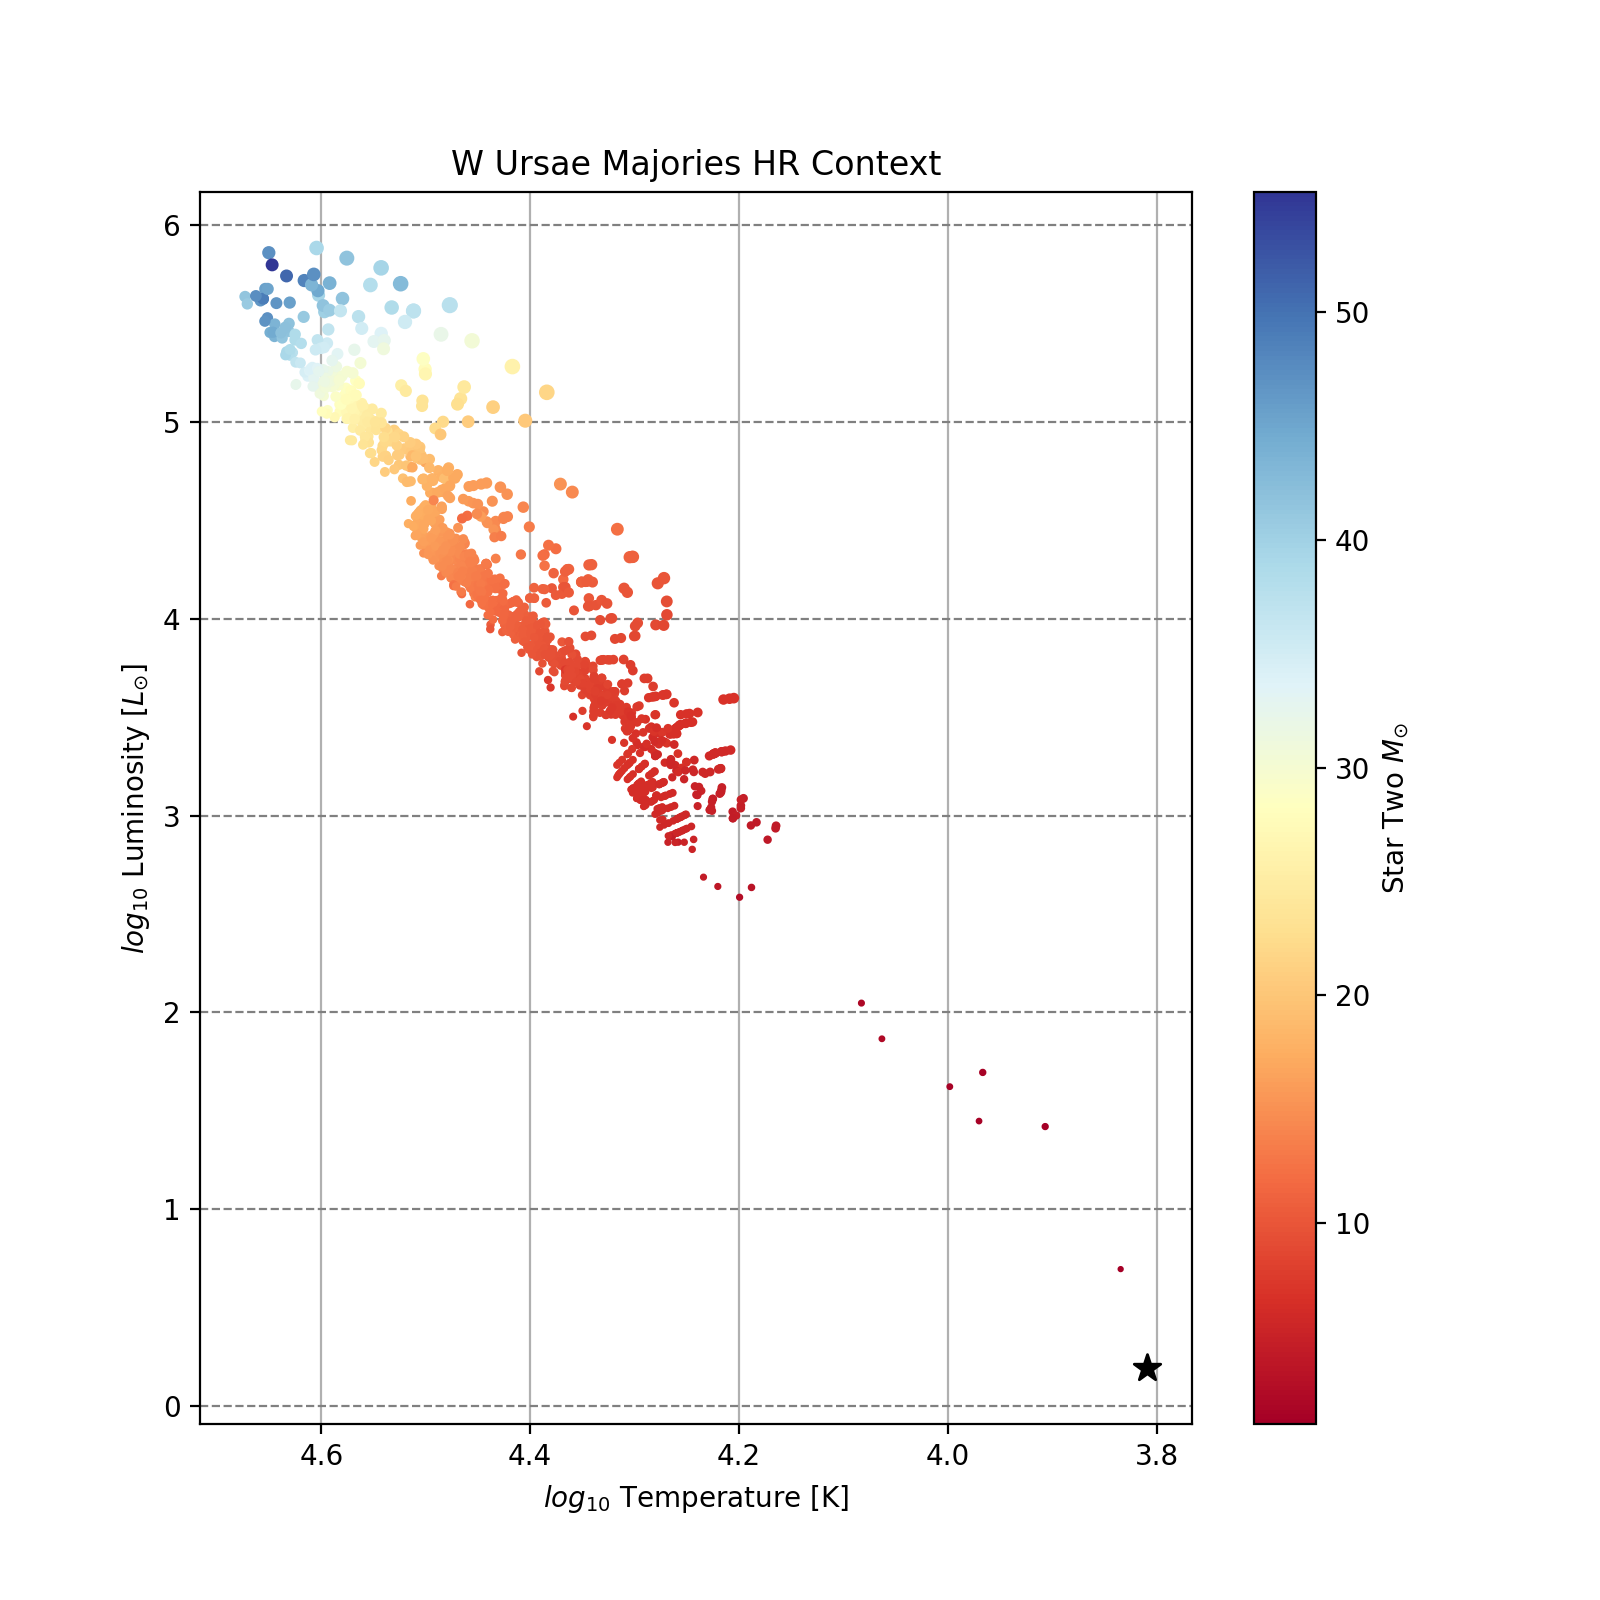
\includegraphics[scale = .6]{figs/GeneratedFigs/W_UMa/WUMaHRDiagram.png}
                \caption{HR Diagram with reference for W UMa using W UMa A. Plotted using data from}
                \label{WUMaResults}
            \end{figure}

            In figure~\ref{WUMaResults} we see that W UMa also follows this linear relationship, however, it has a much lower temperature and luminosity then most of the population. This is a known discrepancy with current simulated models, where simulated values are both typically more luminous and massive than observed~\parencite{Fabry_2025}.

\section{Discussion}   
    Originally I planned on simulating grids for all the types of systems, however, due to time constraints I chose to only focus on one type. This actually tended to be beneficial, as it prevented the scope of the project from becoming too constrained to a singe system.

    \subsubsection{Disclaimers and Notes}
        Due to time constraints, I was not able to cite all the sources within the textbook \parencite{TaurisvandenHeuvel+2023} which I used. This is because it was quite tedious to find the papers themselves within the textbook references and I chose to focus on the content itself instead. 

        Additionally, as this was my first project in \LaTeX (sect.~\ref{LaTeX}) as a freshman, I am sure there are various minor errors and things that do not fit proper convention. Please feel free to reach out with any comments.

    \subsection{Code and Writing Process}
        \subsubsection{Code}

            As I analyzed the data, I found there were certain actions regarding data processing and graphing that I was doing repeatedly, so I wrote a custom Python script in order to streamline the process. This script allowed me to change minor things in the graphs (like the title of color bars) quickly and apply them to all the curated graphs. This script can be found on the GitHub page (sect.~\ref{GitHub}) for the project. 

        \subsubsection{\LaTeX}~\label{LaTeX}
        
            Originally, I started working on this project using Overleaf, however, due the amount of graphs, the time to compile started to rapidly climb up, and eventually I just decided to switch to compiling it locally. On-top of this, I figured I would set up a GitHub in order to additionally push the code and graphs as well. This turned out to absolutely be the right decision, giving me way more freedom.

            Additionally, I wrote the entire paper in \LaTeX, a typesetting system which is the standard for academic papers. I challenged myself to learn and use this format in order to prepare myself for further academia. Using \LaTeX ~also allowed the graphs being generated by my Python scripts to automatically be imported and/or updated into the paper, saving large quantities of time.

        \subsubsection{GitHub} \label{GitHub}
            This essay, the entire paper, all of my data, code, and figures, can all be found on GitHub at \url{https://github.com/PiersonLip/Honors-Independent-Study}. Syncing everything to GitHub additionally allowed me to work on the paper seamlessly from multiple devices, syncing different versions with ease. 

            I worked on this entirely in Virtual Studio Code, as it provided a great environment for me to work efficiently and its integration with Python notebooks and Git helped me work efficiently

\section{Conclusion}
    In conclusion, I found the local populations of V404 Cygni (sect.~\ref{V404Results}), Vela X-1 (sect.~\ref{VelaX1Results}), and W UMa (sect.~\ref{WUMaResults}) by graphing them on HR diagrams in regard to POSYDON data. I found the main causes of mass transfer in detached systems to be wind accretion, semi-detached to be Roche Lobe overflow, and contacts to be direct mass sharing. I found that properties both the graphs in both V404 Cygni (sect.~\ref{V404Results}) and W UMa (sect.~\ref{WUMaResults}) which warrant further investigation.


    \pagebreak
\printbibliography[
heading=bibintoc,
title={\centering Works Cited}
]

\end{document}